\documentclass{article}
\usepackage[unicode]{hyperref}
\usepackage{amsmath,amssymb,graphicx}
\usepackage{tocloft} % برای کنترل بیشتر روی فهرست مطالب
\usepackage{ptext} % فقط برای تولید متن بی‌معنی
\usepackage{placeins} % برای استفاده از \FloatBarrier
% Add required packages BEFORE bidi/xepersian
\usepackage{xcolor}
\usepackage{float}
\usepackage{framed}
\usepackage{lineno}
\usepackage{fancyvrb}
\usepackage{xepersian}
\usepackage{minted} % اضافه کردن بسته minted برای کدها
\settextfont{Yas} % فونت متن فارسی
\setdigitfont{Yas} % فونت اعداد ریاضی

\hypersetup{
    colorlinks=true,
    linkcolor=black,   % رنگ لینک‌های داخلی (فهرست مطالب و ...)
    urlcolor=black,    % رنگ لینک‌های اینترنتی
    citecolor=black     % رنگ ارجاعات (در صورت نیاز)
}


\title{زبان‌های برنامه‌سازی - گزارش فاز ۱}
\author{سهیل محمدخانی، علیرضا کاویانی، سپهر رمضانی
}
\date{} % اگه تاریخ نمی‌خواید، این خط رو فعال کنید

\begin{document}
\maketitle

% فهرست مطالب - با فاصله‌گذاری کمتر
\begingroup
\renewcommand{\baselinestretch}{0.8} % کاهش فاصله بین خطوط
\setlength{\parskip}{0pt} % حذف فاصله بین پاراگراف‌ها
\small % اندازه فونت کوچکتر
\tableofcontents
\endgroup
\newpage % اگر می‌خواهید محتوای اصلی از صفحه بعد شروع شود

\section{تغییرات گرامری}
با توجه به عدم آشنایی با چالش‌های فاز ۱، گرامر دستخوش تغییرات اندکی نسبت به فاز قبلی شد، این تغییرات همه افزایشی بودند 
و هر گرامری که در فاز ۰ گفته شده بوده پیاده‌سازی شده است.\\
همچنین لازم به ذکر است که همه تغییرات گرامری روی 
\lr{predefined statement}
ها بوده‌اند، در زبان طراحی شده، 
\lr{predefined statement}
ها دستوراتی شبیه به تابع هستند که پیاده‌سازی آنها 
\lr{internal}
است و همه آنها با 
\$
شروع می‌شوند، این دستورات عبارتند از:
\begin{itemize}
        \item \$print
        \item \$input
        \item \$set 
        \item \$get 
        \item \$push
        \item \$pop
        \item \textbf{\$size} 
        \item \textbf{\$tocharlist}
\end{itemize}
\
دو دستور آخر که بولد هم شده‌اند، تفاوت گرامر این فاز نسبت به فاز قبل هستند، 
چون این دستورات از نوع اینترنال و پریدیفایند هستند حتما باید در گرامر ذکر شوند.، 
دلیل دستور 
\$tocharlist
این است که استرینگ در زبان ما به طول دیفالت به شکل لیست برسی نمی‌شود، برای همین، برای برسی محتوای آن باید دستوری 
برای کست استرینگ به لیست کاراکترها وجود داشته باشد(نیازی به پریدیفاین کردن کست برعکس نیست چرا که زبان از جمع استرینگ و کاراکتر ساپورت می‌کند و با این عملیات می‌توان کست برعکس را ساخت).
\\
دلیل دستور
\$size
این است که مشابها، اگر ورودی از جنس رشته باشد، برنامه‌نویس هیچ داده‌ای از طول ورودی ندارد،‌ برای همین، حتی با وجود کست به لیست کاراکتر، 
هیچ راهی برای فهمیدن طول رشته ورودی وجود ندارد برای همین \$size لیست نیز باید از قبل در زبان تعریف شده باشد.
\\
طبعا تغییر گرامر موجب تغییر خیلی اندک در پارسر و لکسر زبان هم شد.
\pagebreak
\section{دیتا‌تایپ‌ها}
\subsection{دیتاتایپ‌های اصلی}
برای انتخاب دیتا‌تایپ‌ها مطابق گرامر فاز قبلی عمل شد، دیتا‌تایپ‌های اصلی این زبان عبارتند از:
\begin{enumerate}
        \item int
        \item float 
        \item function 
        \item string
        \item bool 
        \item char
        \item list
\end{enumerate}
همانطور که قبلا هم گفته شد، زبان طراحی شده استرینگ را به چشم یک آبجکت و دیتاتایپ جدا برسی می‌کند، و استرینگ مانند روش مرسوم به چشم یک لیست از 
کاراکتر‌ها 
برسی نمی‌شود و برای تبدیل آن به لیست کاراکتری، باید از پریدیفایند استیتمنت‌ها استفاده کرد.
\\
در فایل
\text{datatype.rkt}
یک تابع جدا به نام 
\texttt{expval->string-for-print}
جز توابع مرسومی که به روش کتاب پیاده‌سازی شده اند نیز وجود دارد که یک داده‌را به ولیو استرینگی برای پرینت کردن آن تبدیل می‌کند، 
این برای این است که برخلاف برخی زبان‌های سطح پایین، داده‌های غیر استرینگی نیز قابل پرینت کردن باشند، البته می‌شد این موضوع را در سمت اینترپرتر هندل کرد اما ترجیح داده شد تا 
در سمت دیتاتایپ‌ها این مورد ذکر شود.
\subsection{دیتا‌تایپ‌های فرعی}
در زبان ذکر شده، جز دیتاتایپ‌های ذکر شده، چند دیتاتایپ دیگر هم اضافه شده که برنامه‌نویس متوجه حضور آنها نیست:
\begin{enumerate}
        \item return 
        \item break 
        \item continue
\end{enumerate}
این دیتاتایپ‌ها در حقیقت دیتاتایپ واقعی نیستند.
\\
در پیاده‌سازی به روشی که کتاب زبان‌ها را برسی می‌کند، پیاده‌سازی زبان‌های فانکشنال کار راحتیست، همچنین زبان‌های سیکونشال نیز 
با ایده‌های کوچک قابل پیاده‌سازی هستند، اما از لحظه‌ای که دستوراتی که پیاده‌سازی یک بلاک را در زمان غیرقابل پیشبینی و در میان بلاک متوقف می‌کنند
که دقیقا ۳ دستور ذکر شده هستند وارد کار می‌شوند، پیاده‌سازی زبان به شدت پیچیده‌ می‌شود و حتی برای پیاده‌سازی این موراد تف‌ها و کار‌های کثیفی انجام داده شد :)
\\
وجود این ۳ دیتاتایپ جزئی از کار‌های کثیفیست که برای پیاده‌سازی عملکرد این ۳ دستور مجبور به انجام آن شده‌ایم است.
\section{تست‌بنچ‌ها}
قبل از توضیح ادامه موارد، نیاز است تا در مورد فرمت تست‌بنچ‌ها توضیح داده شود، 
نتیجه تست‌بنچ ها هم در فایل‌های جدا و هم عکس‌هایی از بخش‌هایی از آن در انتها ضمیمه شده، اما لازم به ذکر است که برای تست کردن فیچر‌های زبان، 
۴ تست بنچ اصلی و چند تست بنچ فرعی نوشته شده است، 
تست‌بنچ های فرعی در کد‌های آپلود شده ضمیمه نشده(چون خیلی کثیف بودند و فقط برای دیباگ از آنها استفاده شد)
اما ۲ تست بنچ اصلی که اولی بسیار کامل است به شرح زیرند:
\subsection{تست‌های ساده}
این تست‌بنچ در فایل 
\texttt{test-basic.rkt}
قرار دارد.
\\
در این تست بنچ، تمام فیچر‌های زبان در کد‌های کوچک مورد برسی قرار گرفتند، این تست بنچ
شامل 
115
تست است، اما هر تست آن در حد ۳ یا ۴ خط کد است و بیشتر برای برسی هر فیچر زبان به صورت جدا و مستقل است.
\subsection{تست‌های سخت}
این تست‌بنچ در فایل 
\texttt{test-hard.rkt}
قرار دارد.
\\
در این تست بنچ، سه برنامه بزرگ نوشته شده که به ترتیب به شرح زیرند:
\begin{enumerate}
        \item محاسبه ۱۰ فیبوناتچی اول به روش تابع بازگشتی برای تست کردن رفتار تابع بازگشتی در شرایط کمی سخت تر از تست‌های عادی
        \item محاسبه ۱۰ فیبوناتچی اول به کمک دیپی، برای تست کردن رفتار دستورات لیستی در شرایط کمی سخت‌تر از تست‌های عادی
        \item پیاده‌سازی یک برنامه برای تبدیل تمام کاراکتر‌های کوچک یک رشته به کاراکتر‌های بزرگ، برای تست کردن رفتار دستورات مرتبط با رشته‌ها در شرایط کمی سخت‌تر از تست‌های عادی.
\end{enumerate}

\subsection{تست‌های ارور هندلینگ:}
این تست‌بنچ در فایل 
\texttt{test-error-handling.rkt}
قرار دارد و برای برسی رفتار زبان در شرایط برخورد با خطای زمان اجرا طراحی‌شده است، لازم به ذکر است برای اجرای این تست‌ها مجبور به استفاده از 
\lr{try-catch}
شدیم چرا که طبق استاندارد داکیومنتیشن، هنگام برخورد با خطا باید برنامه متوقف شود اما تست بنچ باید همه تست‌ها را اجرا کند.
\subsection{تست‌های تایپ‌چکر}
این تست‌بنچ در فایل
\texttt{test-typechecker.rkt}
قرار دارد.
\\
این تست‌بنچ از اینترپرتر مستقل است چرا که تایپ‌چکر جدا از اینترپرتر پیاده‌سازی شده است.
\\
در این مورد بیشتر در بخش تایپچکر صحبت‌کرده ایم.
\subsection{نحوه نمایش نتایج تست‌بنچ‌ها}
نتایج همه تست‌بنچ‌ها هم به صورت فایل و هم به صورت عکس جزئی در بخش جداگانه ضمیمه شده، همچنین 
در هر قسمت، نتایج برخی از تست‌بنچ‌هایی که 
به آن بخش مربوطتند، ضمیمه شده است.
\section{محیط‌ اجرا(environment)}
محیط اجرا تقریبا از تمام توابعی که در کتاب ذکر شده، به علاوه چند تابع جزئی دیگر ساپورت می‌کند، همچنین این محیط در فایل 
\texttt{environment.rkt}
پیاده‌سازی شده.
\\
همچنین در صورت عدم وجود یک متغیر، برسی‌خطا در همین فایل صورت گرفته.
\subsection{\lr{variable management}}
از آنجایی که در فاز گرامر استانداردی در خصوص اسکوپینگ مشخص نشد، زبان ما از لحاظ گرامری طوری طراحی شده که همه متغیر‌ها لوکالند و متغیر گلوبالی وجود ندارد، 
طبعا چنین چیزی در روند اجرا تاثیرگزار نیست، همچنین لازم‌ به ذکر است که برای تغییر گرامر برای ساپورت متغیر گلوبال، باید تغییرات زیادی در فاز ۰ صورت می‌گرفت و می‌بایستی این مورد در فاز قبل ذکر می‌شد.
\\
ذخیره‌سازی متغیر‌ها از هر نوعی به خصوص از انواع گفته شده در زبان قابل انجام است.
\\
همچنین امکان شدو نیز وجود دارد،
چون منابع پس از خارج شدن از هر اسکوپ آزاد می‌شوند، 
برای ساپورت شدو کافی بود تا تنها آخرین مقدار از یک اسم در انوایرمنت خروجی داده شود.
\begin{figure}[h]
        \centering
        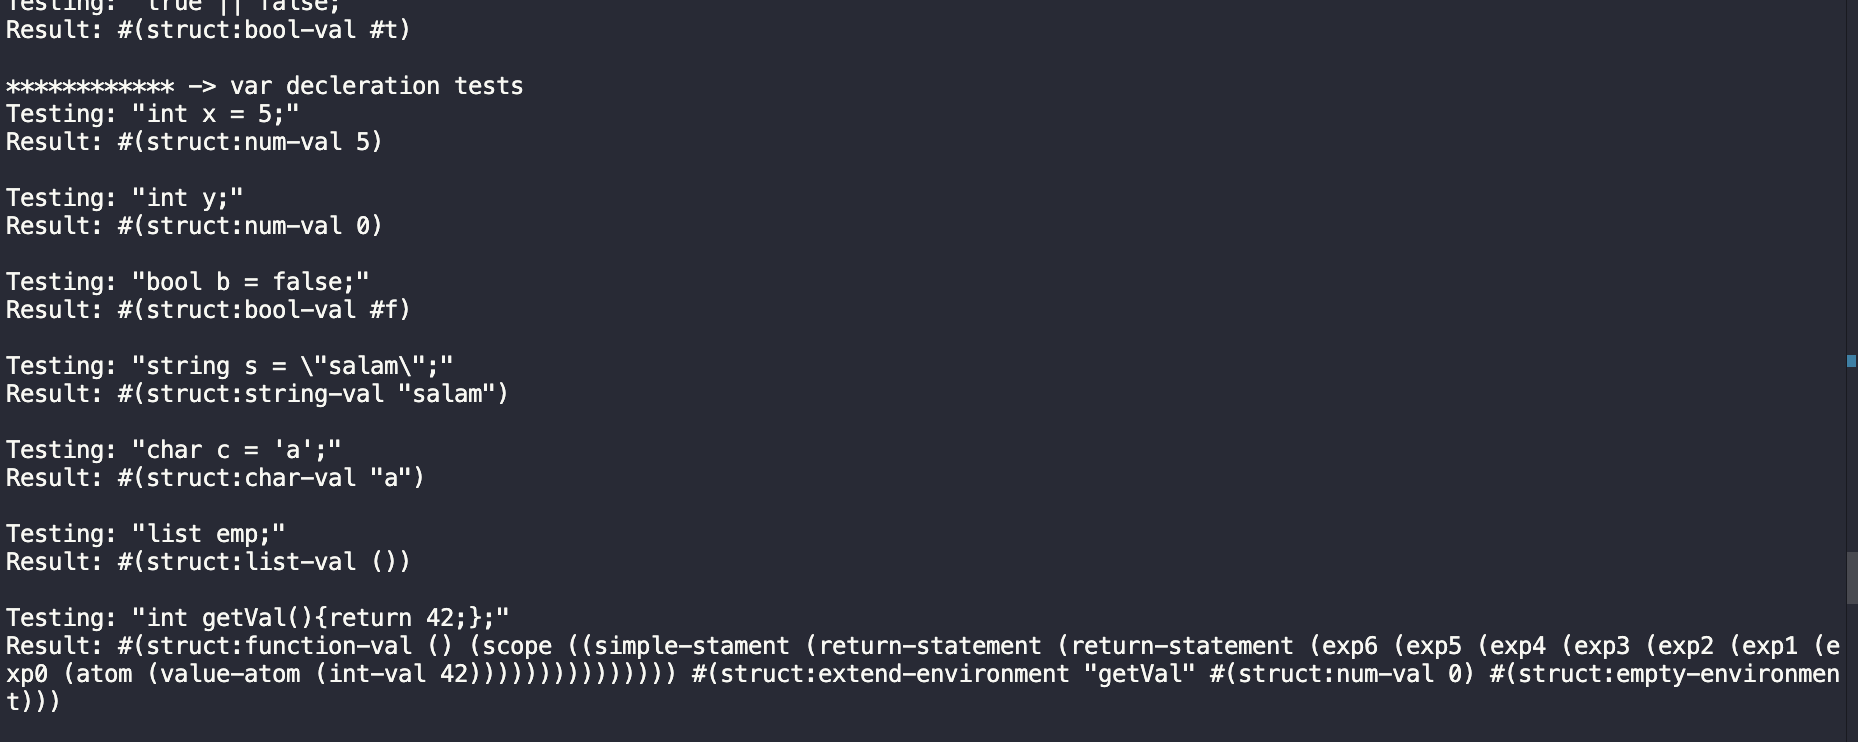
\includegraphics[width=1\linewidth]{pics/var1.png}
        \caption{بخشی از تست‌بنچ ساده، همچنین لازم به ذکر است مقدار دهی اولیه به لیست در زبان برای‌ ساده‌سازی ممکن نیست و باید با push های متوالی اینکار انجام شود.}
\end{figure}
\subsection{\lr{function handling}}
توابع مانند روش کتاب، به چشم یک متغیر دیده می‌شوند، همچنین با استفاده از روشی مانند روش کتاب برای پیاده‌سازی 
\lr{letrec}
امکان تعریف تابع بازگشتی نیز وجود دارد.
\begin{figure}[h]
        \centering
        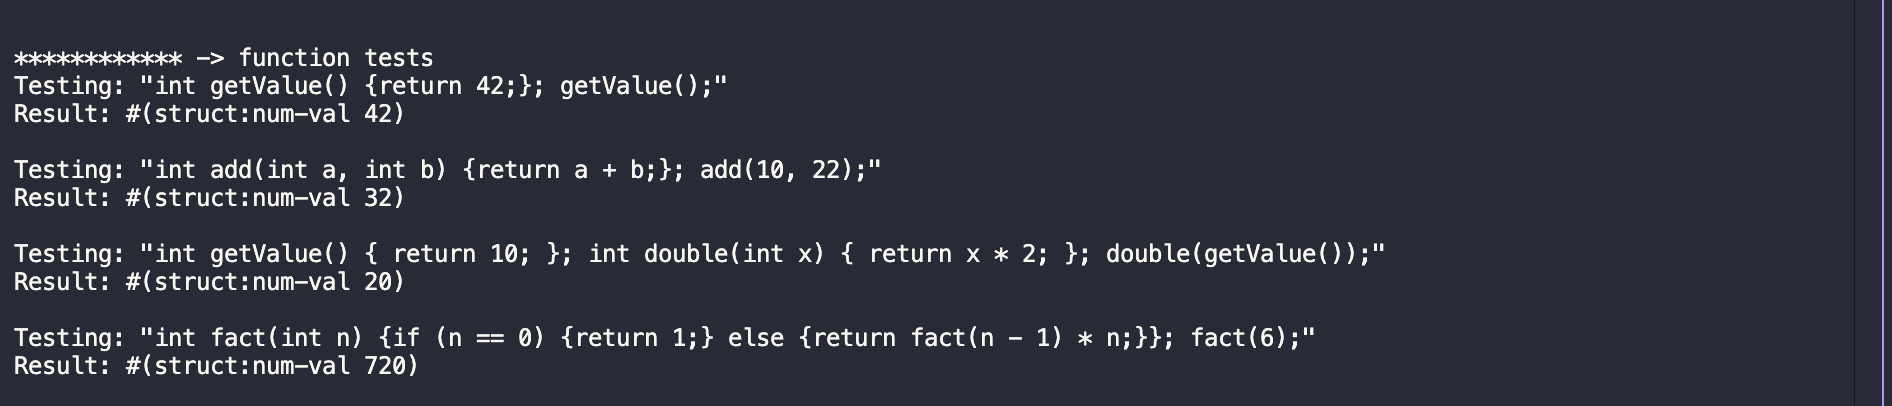
\includegraphics[width=1\linewidth]{pics/func1.png}
        \caption{بخشی از تست‌های ساده برای توابع}
\end{figure}
\subsection{\lr{Lazy Evalutation}}
دقیقا استراکچر‌‌هایی مانند 
\lr{thunk}
در زبان پیاده‌سازی نشده، اما سعی شده اگر می‌شد، در محاسبه 
\lr{value-of}
هر نود 
\lr{AST}
اگر بچه سمت چپ کافی بود، بچه سمت راست را حساب نکنیم(تنها در آپریشن‌هایی که شبیه سی، به صورت لیزی ایولیویت می‌شوند، طبعا این روش کارایی شبیه \lr{thunk} را ندارد اما اندکی به بهبود زمان اجرا کمک می‌کند.)
\subsection{\lr{Memory Management}}
همه منابع داخل اسکوپ تعریف شده و خارج اسکوپ غیر قابل دسترسی هستند.
\section{ارزیابی عبارات}
تمام عبارات در گرامر پیاده‌سازی شده‌اند، 
این عبارات همه عبارات گفته شده در داکیومنتیشن و حتی مقدار خیلی بیشتری را تشکیل می‌دهند، تنها استثنا، عبارت
\texttt{for}
است که چون در اسپسیفیکیشن فاز قبل، تنها ذکر شده بود که نیاز است از یک نوع حلقه فارغ از نوع آن ساپورت کنیم، هم در فاز گرامر و هم در این فاز از 
حلقه فور صرف نظر کردیم چرا که پیاده‌سازی آن بسیار پیچیدگی به کد اضافه می‌کند و همچنین 
صرفا با داشتن 
\lr{while}
می‌توان تمام عملیات‌های فور را انجام داد.
\subsection{توابع مهم در پیاده‌سازی اینترپرتر}
صرفا لازم به ذکره جاهایی که میبینین نوشته شده 
\lr{tof}
سر اینه که سر پیاده‌سازی وایل مشکلای خیلی عجیبی خوردیم و مجبور شدیم تقریبا کل توابعمونو یکم عوض کنیم که اوکی باشند، سر همین تو ورژن قبل پاک کردن تابعای به درد نخور 
هر تابع ۲ تا ورژن داشت وگرنه دلیل دیگه‌ای نداره
\begin{itemize}
        \item value-of-x: این تابع مانند کاریست که کتاب در طراحی زبان let انجام داد، این تابع، یک نود \lr{AST} به تایپ \lr{x} را روی محیط $p$ ایولیویت کرده و نتیجه را بر می‌گرداند.
        \item exec-statement-list-tof: این تابع یک لیست از دستورات را گرفته و آنها را به ترتیب و به صورت سیکونشال اجرا کرده و در صورت نیاز تغییراتی روی انوایرمنت می‌دهد، این تابع دقیقا 
        نقطه ایست که پیاده‌سازی تقریبا غیرخطی کتاب را تبدیل به یک پیاده‌سازی خطی و سیکونشال می‌کند(مانند تمرینی که در آن خواسته شده بود تا begin را پیاده کنیم)
        \item get-default-value: مقادیر دیفالت برای تایپ‌های متفاوت را خروجی می‌دهد
        \item extract-var-name: نام متغیر از نود \lr{AST} مشخص می‌شود.
        \item exec-function-decleration-unified: تقریبا مشابه عملکرد \lr{letrec}
        \item bind-parameters: لیست پارامتر‌های یک تابع را گرفته و با نگاه به انوایرمنت، بایندینگ‌های مورد نظر را انجام می‌دهد
\end{itemize}
همچنین جدای از پیاده‌سازی برای 
\lr{valud-of-x}
برای گرامر‌هایی که ساپورت کرده‌ایم، 
برای پریدیفایند استیتمنت‌ها هم هر یک پیاده‌سازی مشخصی انجام شده تا زبان یک زبان تورینگ کامپلیت شود.
\subsection{عبارات پایه}
پیاده‌سازی عبارات پایه چلنج خاصی نداشت، برای عبارات ریاضی با توجه به گرامر ترتیب عملیات‌ها به درستی انجام می‌شود و در اینترپرتر صرفا باید عملیات مورد نظر را اناجم دهیم که کار ساده‌ایست، 
\begin{figure}[h]
        \centering
        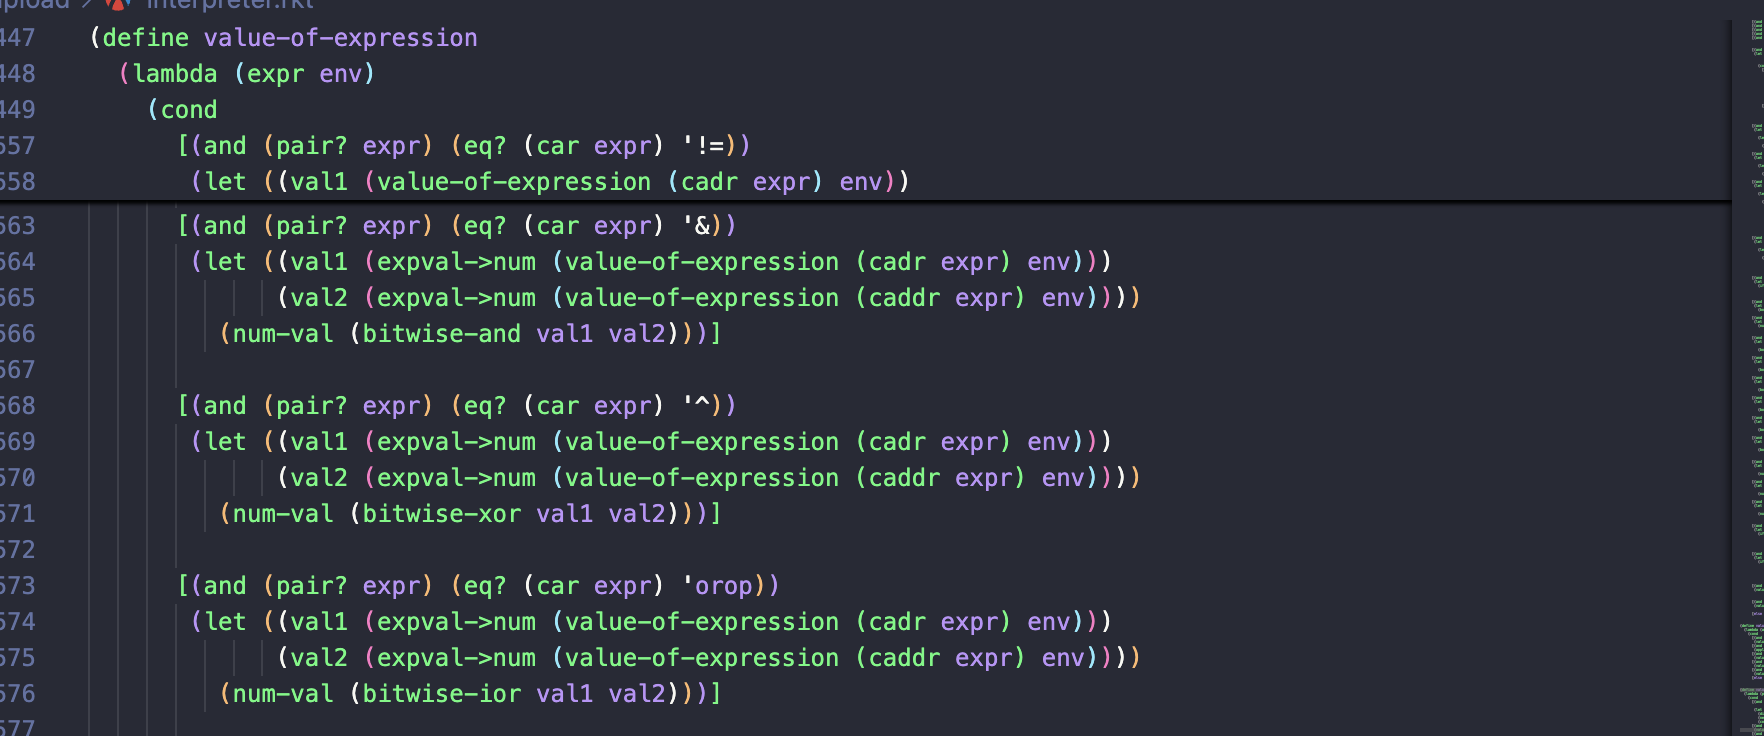
\includegraphics[width=0.5\linewidth]{pics/t1.png}
        \caption{نمونه‌ای از پیاده‌سازی چند آپریشن از آپریشن‌های ذکر شده:}
\end{figure}
\begin{figure}[h]
        \centering
        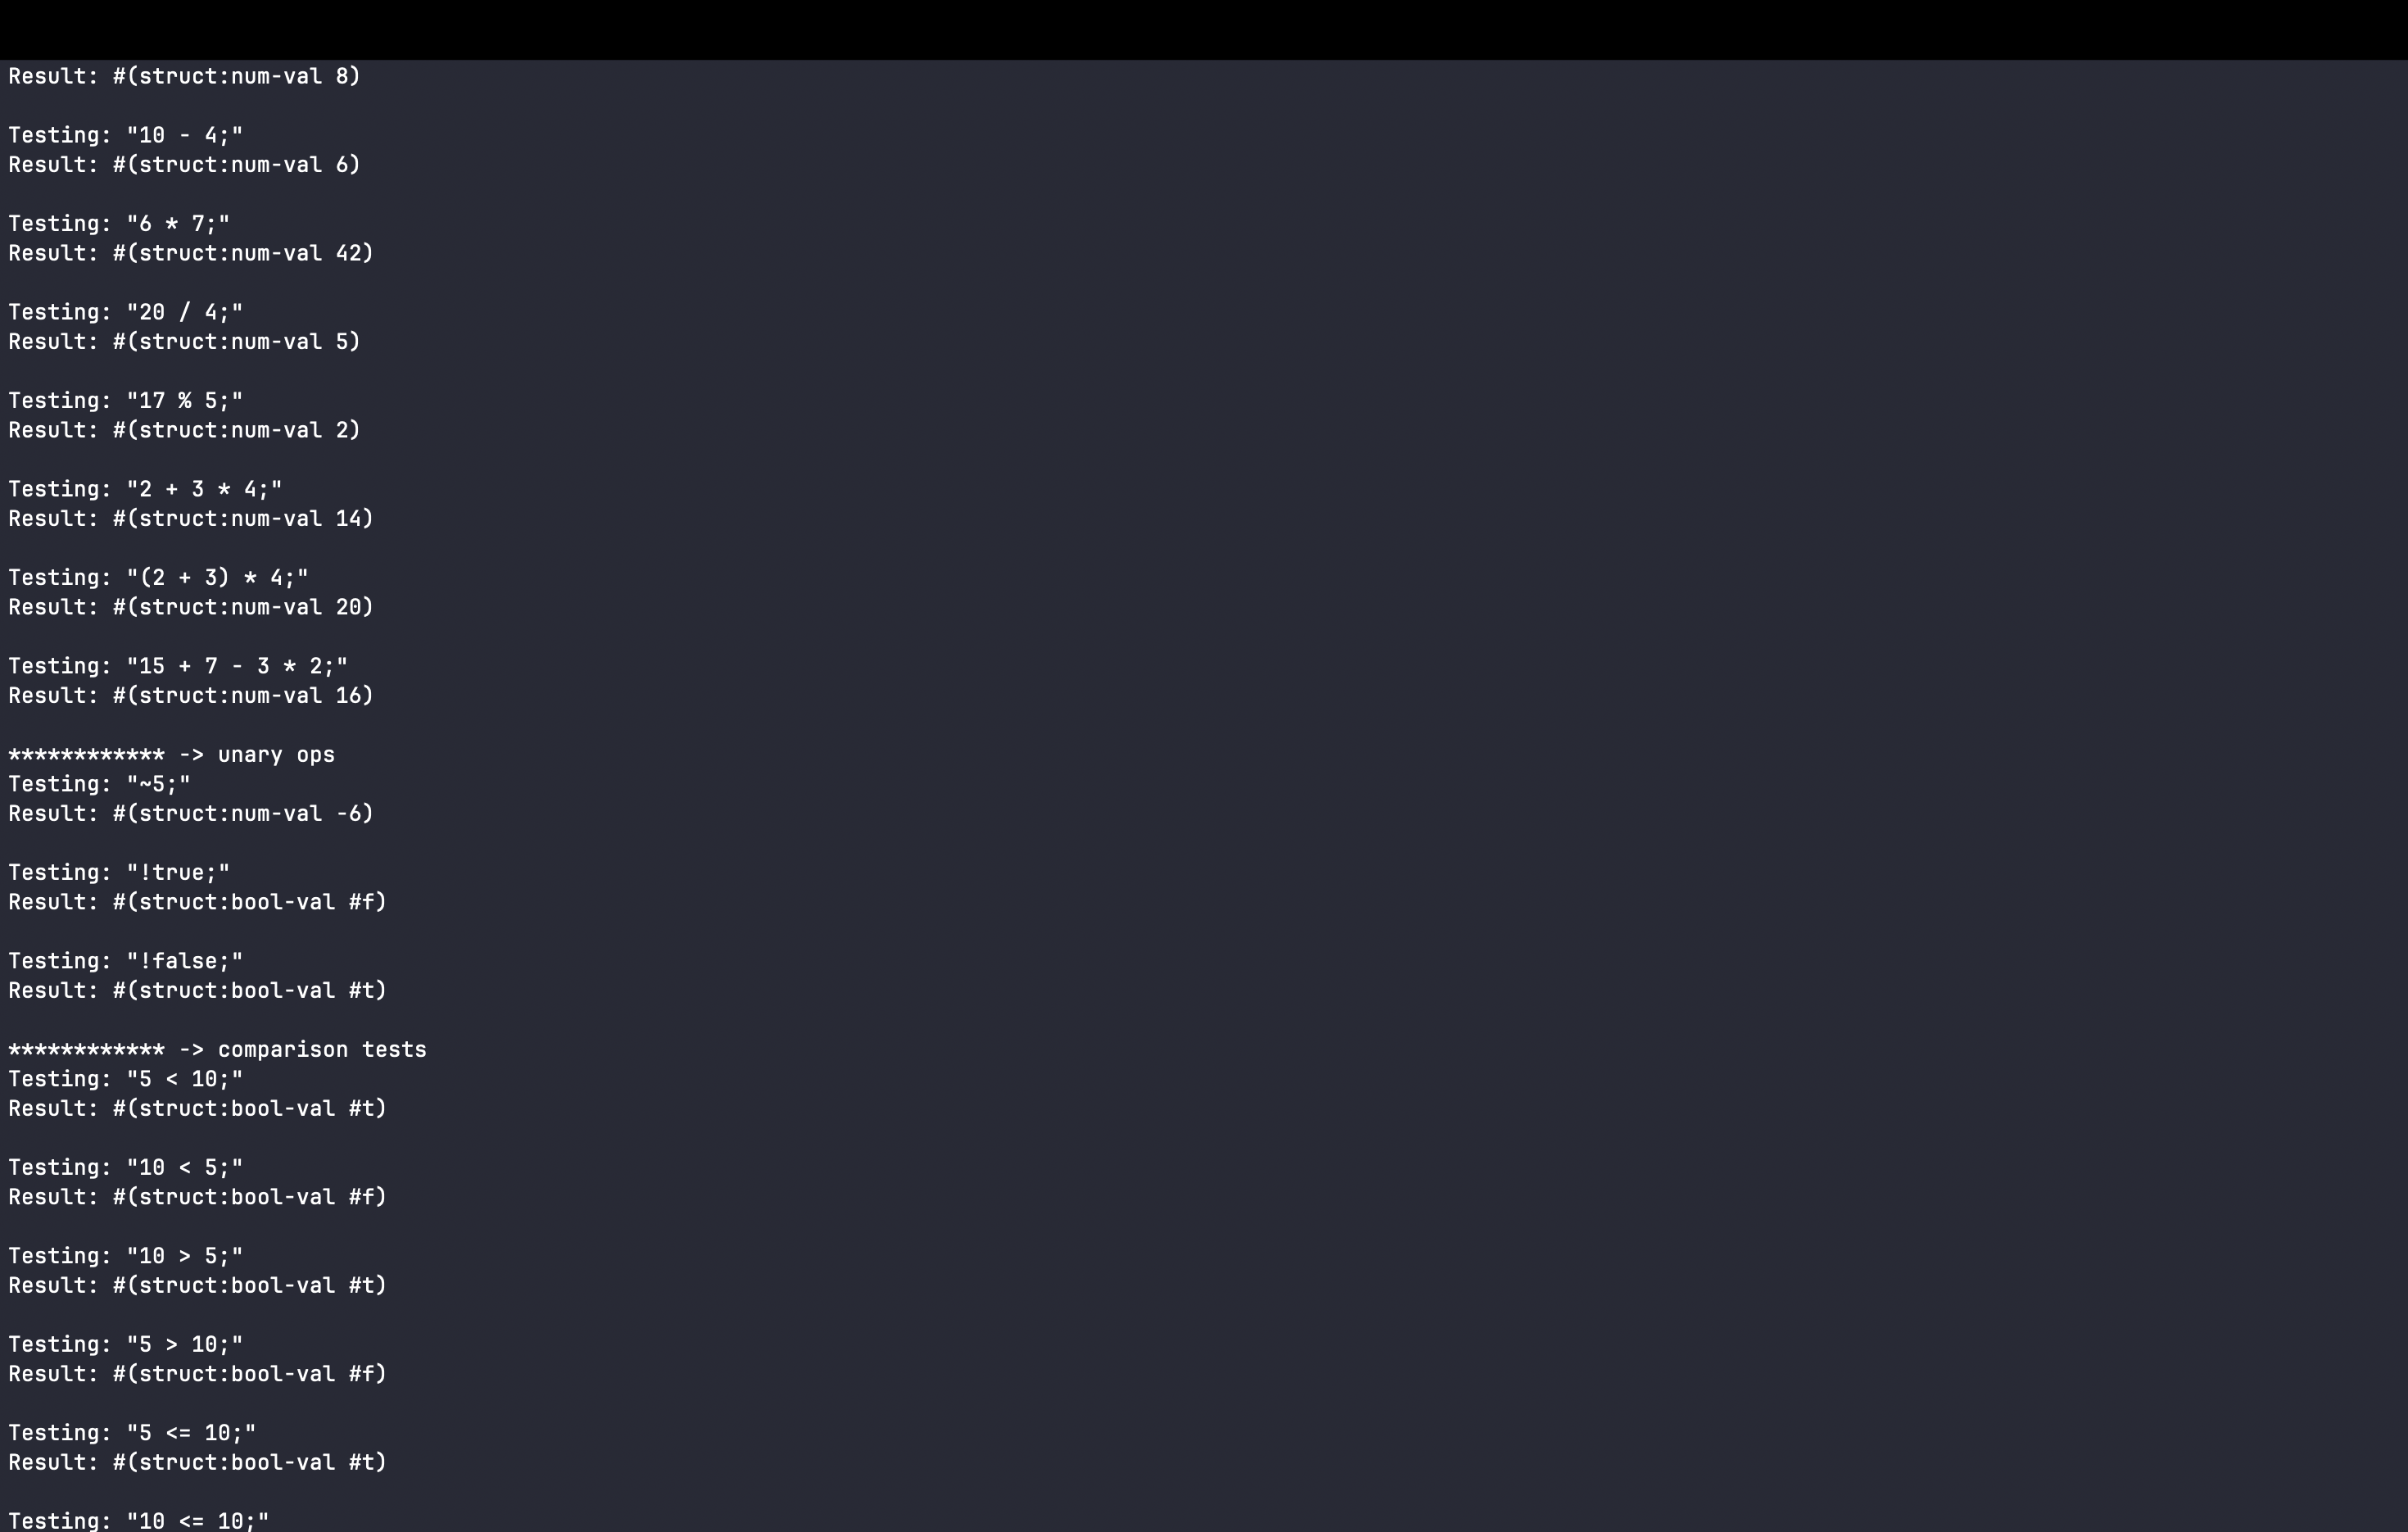
\includegraphics[width=0.5\linewidth]{pics/t2.png}
        \caption{بخشی‌از تست‌های عملیات‌های پایه:}
\end{figure}
\FloatBarrier
\subsection{ساختار کنترلی}
\begin{itemize}
        \item if-else:
        برای بلوک ایف خالی یا ایف الس، با داشتن ولیو‌آف بچه متناظر با کاندیشن، ادامه کار تنها گرفتن ولیو‌اف بچه‌ایست که طبق ولیو کاندیشن باید اجرا شود است،
        به عبارت دیگر،‌ بجز حالت بندی روی نوع بلاک ایف و کثافت کاری‌های اینچنینی، کل کد مربوط به ایف در ۲ خط زیر قابل خلاصه است:
        \begin{minted}{racket}
        (if condition-val
             (exec-statement-tof then-scope env)
             (exec-statement-tof else-scope env))
        \end{minted}

        \begin{figure}[h]
        \centering
        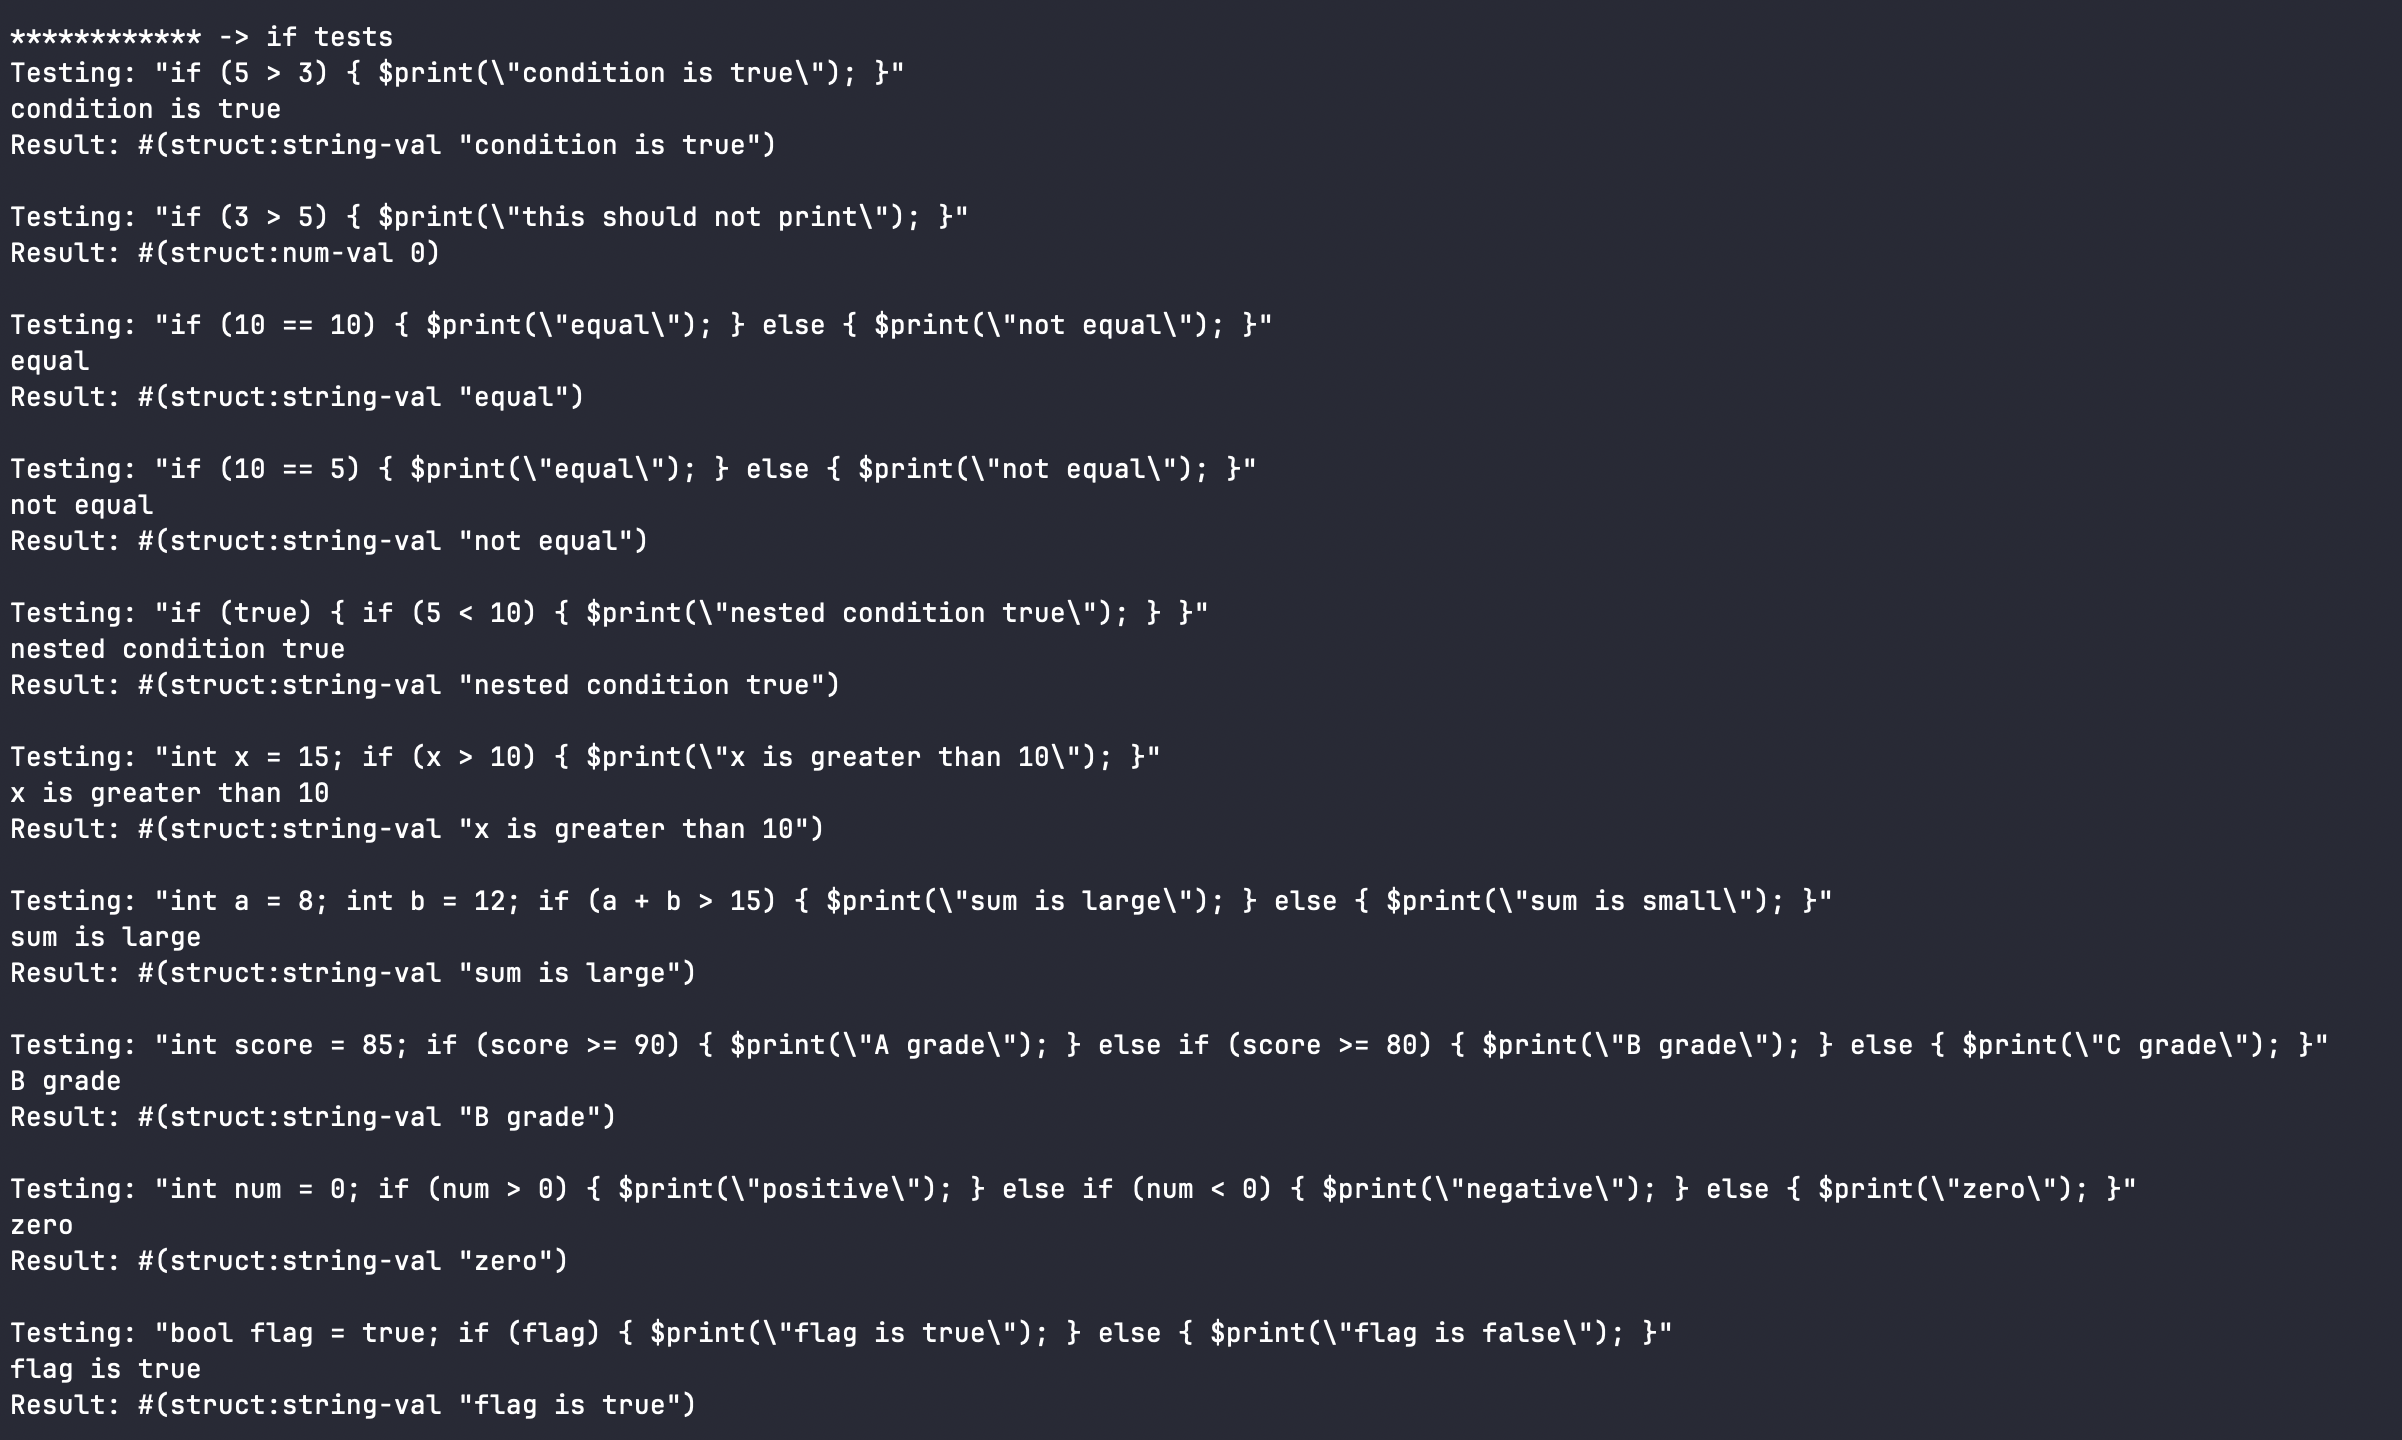
\includegraphics[width=0.5\linewidth]{pics/tif.png}
        \caption{تست‌های ایف:}
\end{figure}
\FloatBarrier
        \item while:
        برای وایل، 
        از ساختار زیر برای ساپورت آن استفاده شد:
        \begin{minted}{racket}
(define exec-while-loop-tof
  (lambda (condition body-scope env)
    (let ((condition-val (expval->bool (value-of-expression condition env))))
      (if condition-val
          ; Expained Later:
          (cons (num-val 0) env)))))
        \end{minted}


قسمت خالی گذاشته شده، اگر از کانتینیو و برک ساپورت نمی‌کردیم، بسیار راحت قابل پیاده‌سازی بود اما دقیقا بخاطر ساپورت ازز کانتینیو و برک و مشکلاتی که در 
کنترل فلو ساده برنامه به وجود می‌آمد، این تیکه بسیار پیچیده و طولانی شد.
        \begin{figure}[h]
        \centering
        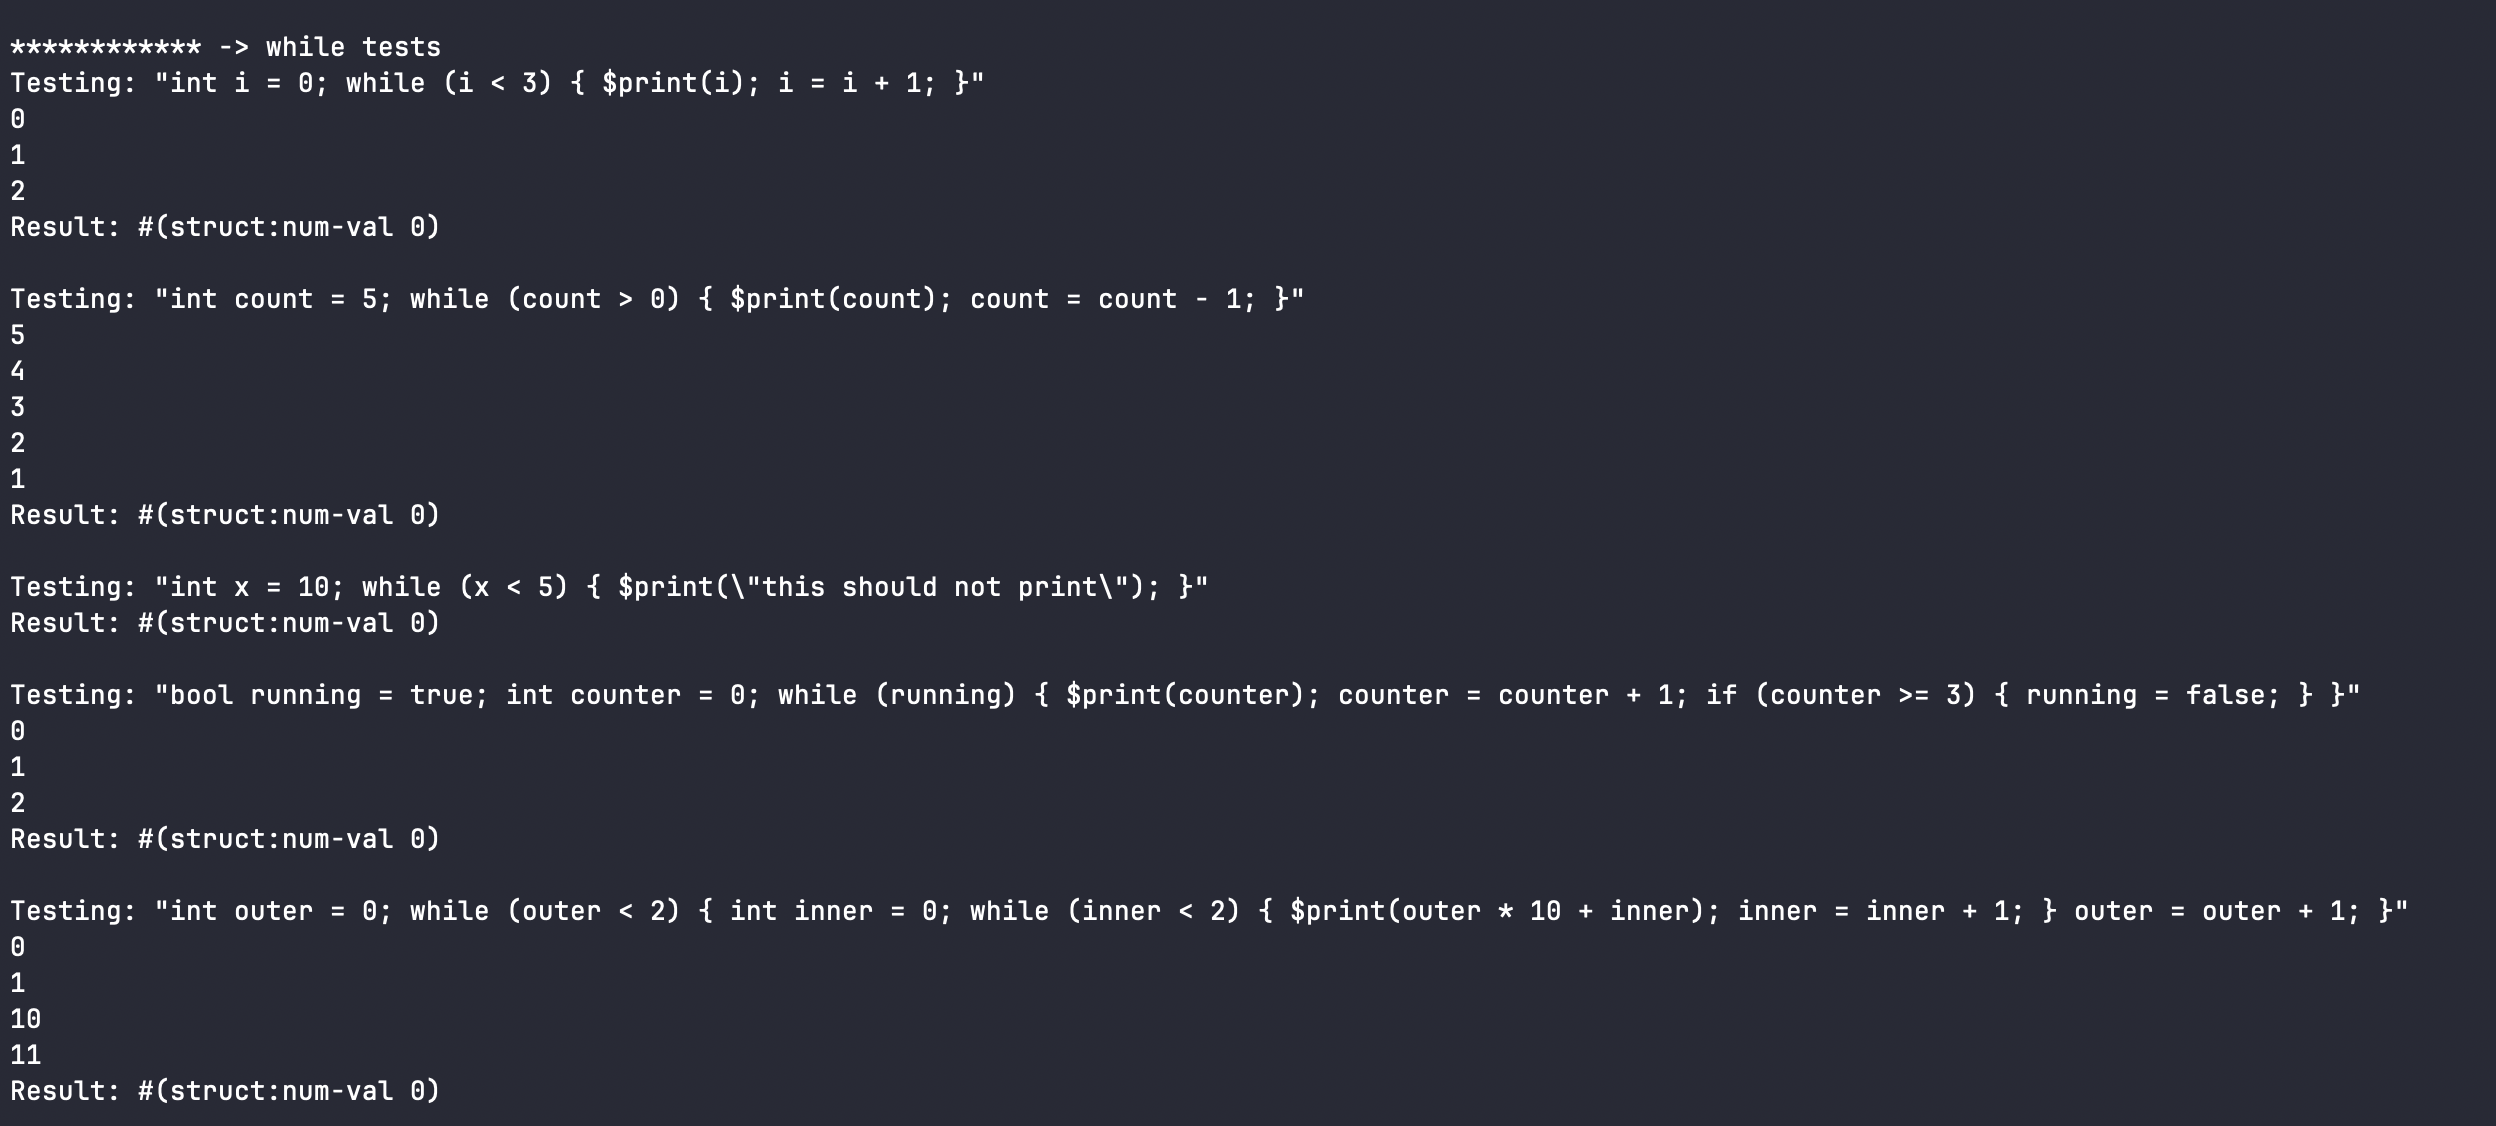
\includegraphics[width=0.5\linewidth]{pics/twhile.png}
        \caption{بخشی از تست‌های وایل:}
\end{figure}
\FloatBarrier
\end{itemize}
\subsection{توابع}
در زبان ما توابع
member 
های درجه اول هستند و در انوایرمنت تفاوتی با متغیر‌ها ندارند،
هرچند امکان پاس دادن تابع در زبان تعبیه نشد اما با تغییرات خیلی خیلی کم بخاطر نوع پیاده‌سازی، 
امکان این امر نیز ممکن می‌شود.
\\
همچنین برای ساپورت از توابع بازگشتی، از تکنیکی مشابه لترک در کتاب استفاده شد\\
برای پیاده‌سازی توابع، ابتدا تابع 
\lr{bind-parameters}
پیاده‌سازی شد که برای بایند کردن پارامتر‌های مورد نیاز تابع با مقادیر موجود در انوایرمنت و درست کردن انوایرمنت مخصوص اسکوپ درون تابع است، 
همچنین، یک تابع دیگر به نام 
\lr{extract-parameters-names}
پیاده شده که نام پارامتر‌های تابع را خروجی می‌دهد.
همچنین دوتابع برای ادامه کار پیاده شد، یکی 
\lr{exec-function-declaration-tof}
که یک تابع را با تکنیکی مشابه لترک، در انوایرمنت تعریف می‌کند(و اسکوپ و نام و ریترن تایپ و پارامتر‌های آن را نیز در کنار آن ذخیره می‌کند)
و دیگری 
\lr{value-of-function-call}
که تابع را فراخوانی کرده و حاصل فراخانی را خروجی می‌دهد.
تست های مربوط به فانکشن ها قبلا در قسمت‌های قبل(شکل ۲)
ضمیمه شده بود و دوباره آن‌را ضمیمه نمی‌کنیم(همچنین از دایرکتوری results نتیجه همه تست‌ها قابل مشاهده‌است.)
\subsection{داده‌ساختار‌ها(لیست)}
تنها داده‌ساختار پیچیده که به صورت تایپ پریدیفاین شده در زبان 
وجود دارد لیست است تا زبان به یک زبان تورینگ کامپلیت تبدیل شود(لیست یا ارایه برای بازی کردن نقش تیپ در یک ماشین تورینگ ضروریست)
\\
برای سادگی، در زبان ما نمی‌توان مقدار اولیه به لیست داد و با دستور پریدیفایند 
\texttt{\$push}
می‌بایستی مقادیر اولیه را پس از تعریف یک لیست تهی، یکی یکی به آرایه پوش کرد، برای تعریف لیست کار عجیبی انجام نشد، دیتاتایپ لیست درون خود به عنوان ولیو 
یک لیست از جنس لیست رکت نگه می‌دارد و پریدیفایند استیتمنت های 
get, set, push, pop
به کد رکت روی لیست درونی تبدیل می‌شوند.
\\
به عنوان مثال، کد گت یا همان ایندکسینگ با پاک کردن موارد مربوط به ارور هندلینگ به کد ساده زیر تبدیل می‌شود:
\begin{minted}{racket}
            (let ((list-expval (apply-env var-name env))
          (index-val (value-of-expression index-expr env)))
\end{minted}
که 
\texttt{index-val}
از توابع اینترنال رکت است.
\\
\textbf{دقت کنید که ایندکسینگ به صورت اپریتوری در زبان وجود ندارد و بجای آن پریدیفایند استیتمنت گت وجود دارد که نقش ایندکسینگ را ایفا می‌کند.}
        \begin{figure}[h]
        \centering
        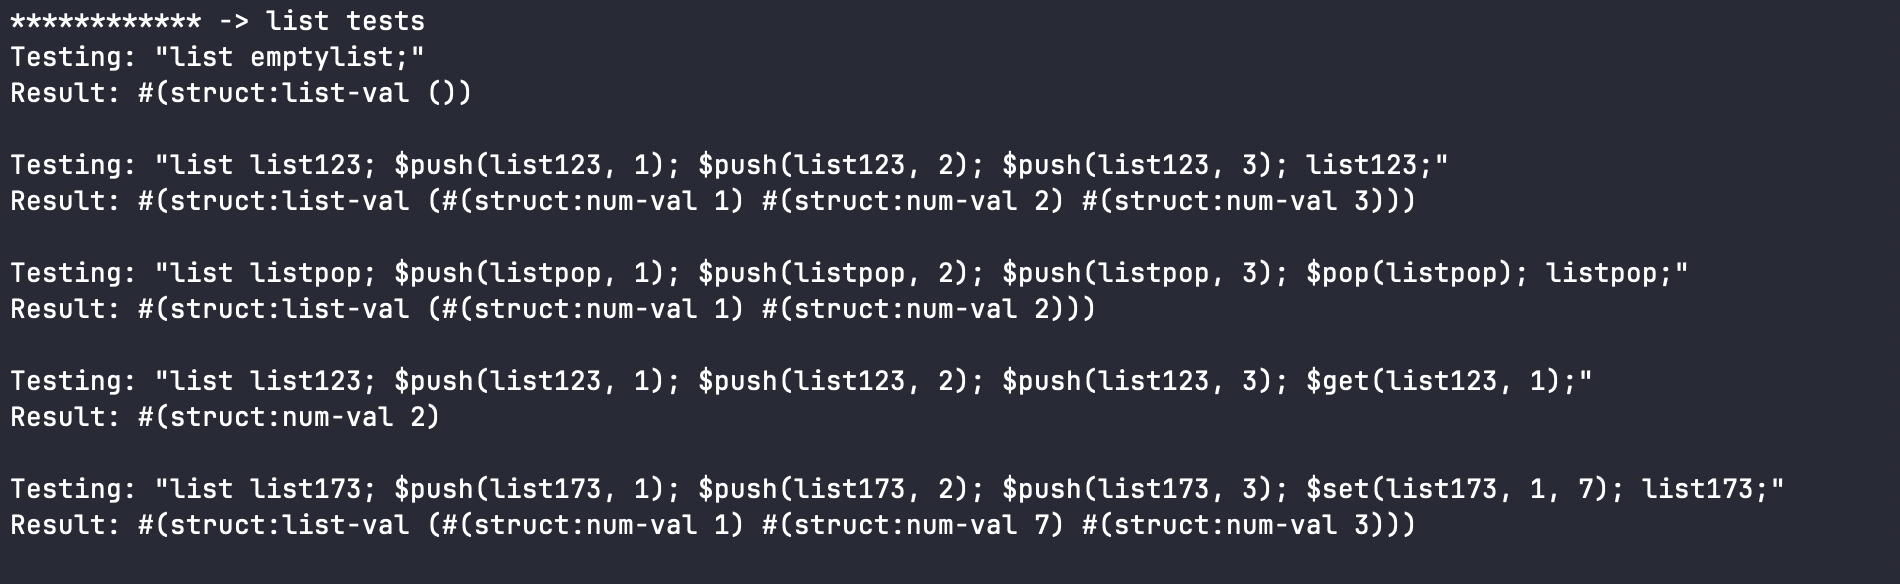
\includegraphics[width=0.5\linewidth]{pics/list.png}
        \caption{تست‌های ساده مربوط به لیست}
\end{figure}
\FloatBarrier
\subsection{ورودی، خروجی، و سایر پریدیفایند استیتمنت‌ها}
پیاده‌سازی پریدیفایند استیتمنت ها صرفا معادل این بود که یک کد رکت برای برخی از توابع بزنیم تا بتوان سایر کد ها را به کد‌های مرتبط به زبان ترجمه کرد، به عبارت دیگر، این توابع تنها برای تورینگ کامپلیت کردن زبان بودند،.
\\
برای پیاده‌سازی پرینت، می‌بایستی تابعی می‌زدیم که یک دیتاتایپ که در پیاده‌سازی رکتی همیشه از جنس استراکت است را تبدیل به 
استرینگ می‌کردیم که در قسمت دیتاتایپ‌ها توضیح داده شد، چالش دیگری در این قسمت نبود، برای مثال، یکی از این پیاده‌سازی ها را ضمیمه کرده‌ایم:
        \begin{figure}[h]
        \centering
        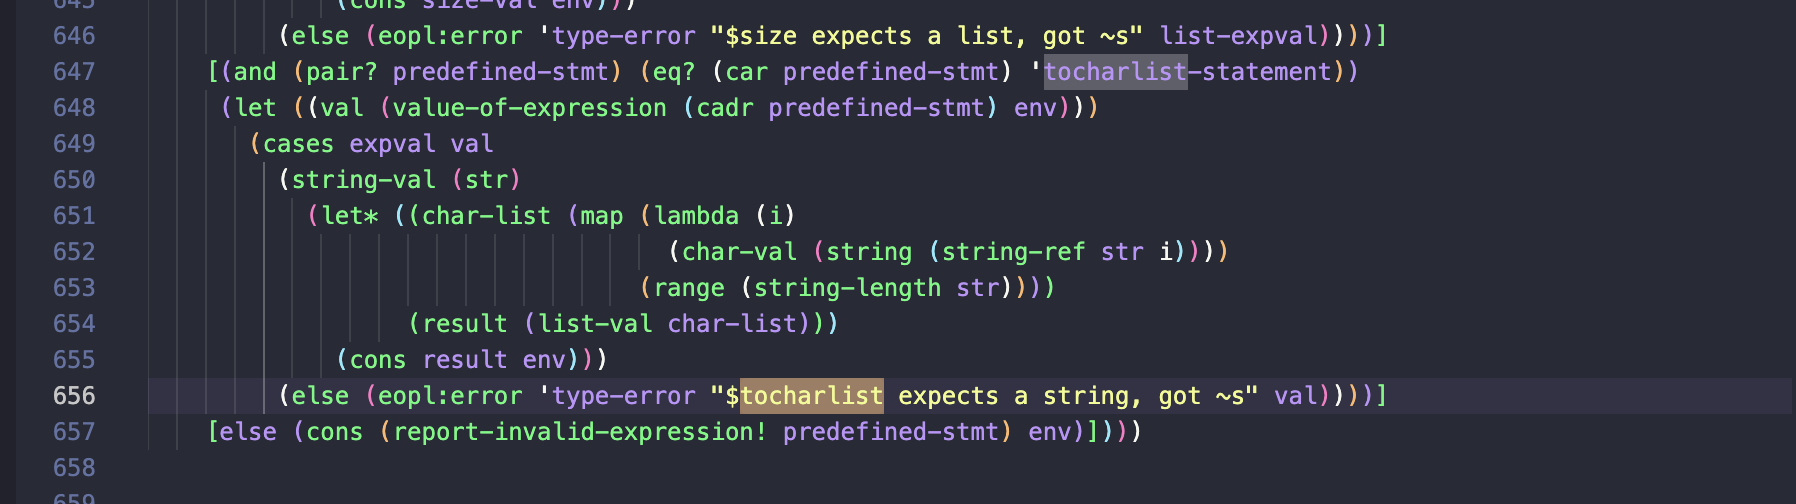
\includegraphics[width=0.5\linewidth]{pics/tch.png}
        \caption{پیاده‌سازی دستور tocharlist که یک استرینگ را به لیست کاراکتر تبدیل می‌کند(چون استرینگ در زبان ما از جنس لیست نیست)}
\end{figure}
\FloatBarrier
\section{مدیریت خطا}
برای مدیریت خطا، از کتاب‌خانه 
\lr{eopl}
استفاده شده، همچنین به علت تایپ استریکت بودن زبان پیاده‌سازی شده، مدیریت‌ خطا‌ها کمی آسان‌تر از حالت عادی‌ است.
\\
برای مدیریت خطا، جز ۲ مورد(یکی در برای گرفتن مقدار وریبلی که در انوایرمنت نیست و دیگری و دیگری برای کستینگ ناموفق در دیتاتایپ‌ها)
همه خطا‌ها مربوط به اکسپرشن ایولیویشن هستند، و به راحتی حین ایولیوت کردن، قابل پیشبینی هستند، برای مثال وقتی 
\lr{valud-of}
برای اکسپرشن از نوع تقسیم پیاده‌سازی می‌شود، کافیست تا اگر ولیو‌آف سمت راست ۰ بود، توسط 
\lr{eopl::error}
خطای دیویژن بای زیرو داده شود.
\\
هنگام بروز خطا نوع خطا و همچنین پیام مرتبط با آن نمایش‌داده می‌شود و اجرای برنامه متوقف می‌شود، نتایج تست بنچ ارور هندلینگ در زیر آمده که نشان می‌دهد 
همه خطا‌هایی که در داک ذکر شده بود برسی شده‌اند، همچنین، خطا‌های بیشتری فرای آنچه در داک گفته شده، پیاده‌سازی شده‌اند.
\\
\begin{figure}[h]
        \centering
        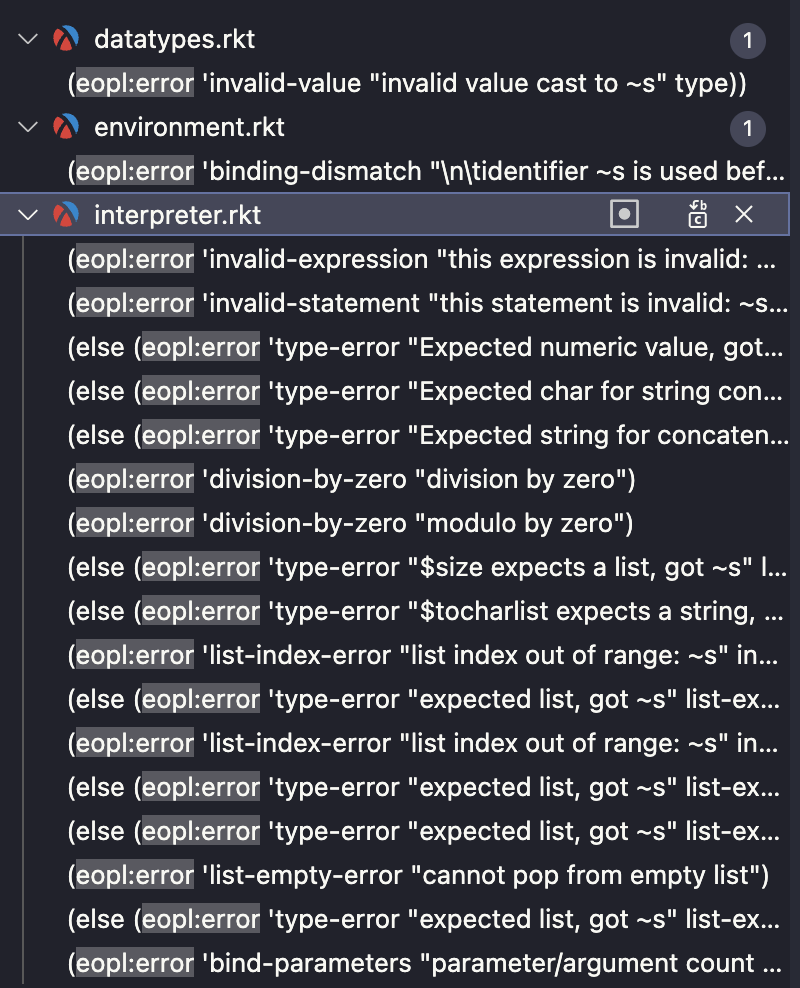
\includegraphics[width=0.5\linewidth]{pics/eopl.png}
        \caption{تمام‌ خطا‌هایی که در زبان از آنها ساپورت می‌شود}
\end{figure}

\begin{figure}[h]
           \centering
        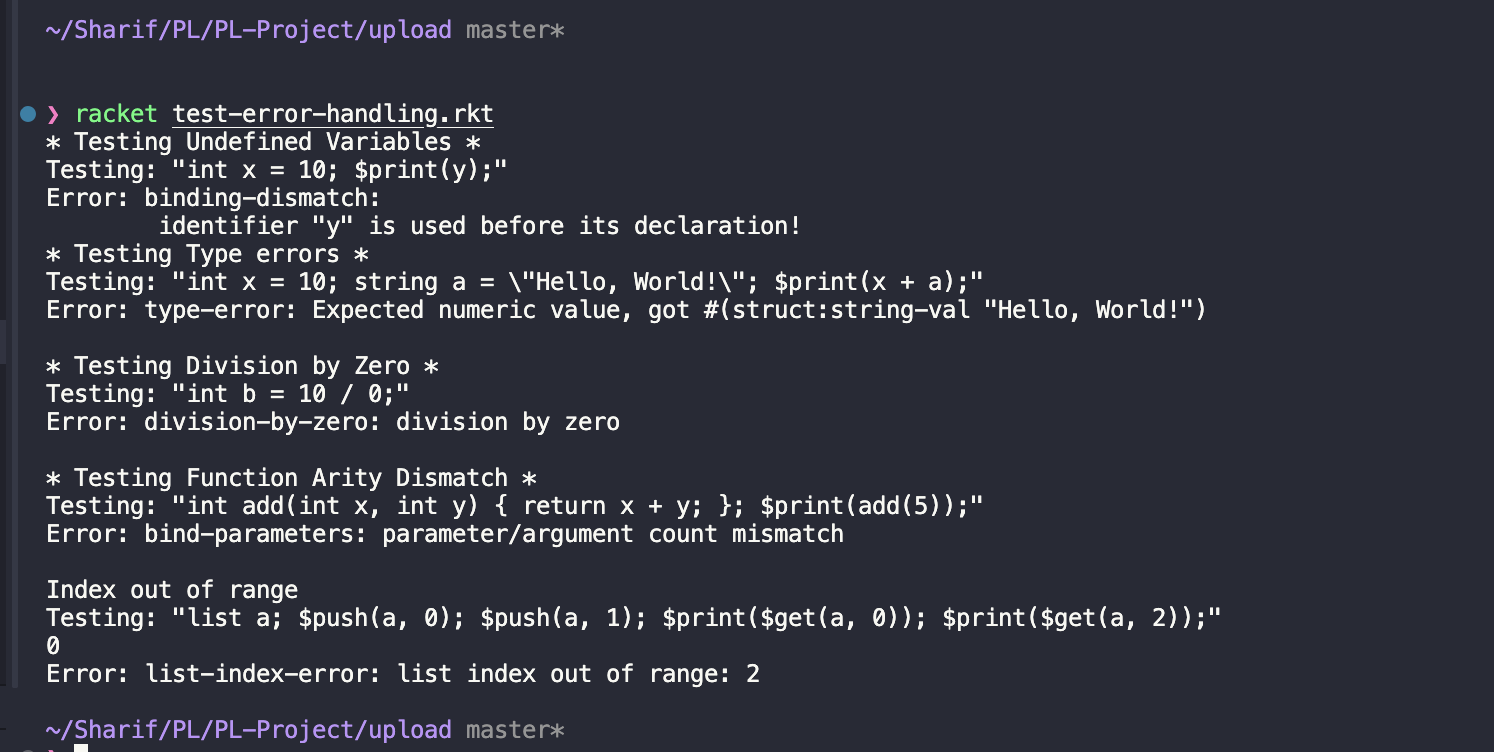
\includegraphics[width=1\linewidth]{pics/error-tb.png}
        \caption{نتیجه تست بنچ ارور هندلینگ، دقت کنید اجرای هر برنامه در این تست بنچ در یک ترای‌کچ قرار دارد تا در صورت بروز خطا، برنامه متوقف نشود و همه تست‌ها اجرا شوند.}     
\end{figure}
\FloatBarrier
\section{TypeChecker}
\textbf{دقت کنید که برای سادگی، یک محیط برای تایپ چک کردن و اینترپرت بعد آن ساخته نشده و این دو مستقل از هم عمل می‌کنند، برای همین برای 
اجرای کد، ابتدا باید یک بار به صورت دستی تایپ چکر را روی آن در صورت نیاز از اطمینان از لحاظ تایپ‌ها ران کنیم و سپس اینترپرتر را روی آن اجرا کنیم، 
البته که تایپ‌ارور ها به طول جداگانه در اینترپرتر جلوی بسیاری از خطا‌های تایپی را بدون اجرای تایپ‌چکر می‌گیرند.
}
همانطور که قبلا هم گفته‌شد، زبان طراحی شده زبان تایپ استریکت است و تمام تایپ‌ها به خصوص در ورودی و خروجی توابع، 
تایپ‌ها کاملا مشخص شده اند و گرامر به طوری طراحی شده که زبان تایپ استریکت باشد. برای همین، 
نیازی به پشتیبانی از 
\lr{type inference}
نیست و تمام متغیر‌ها بدون نیاز به استنتاج ثانویه، از همان اول تایپ مشخص دارند.
\\
پس می‌توان صرفا با تایپ چکینگ عادی بدون حل یک دستگاه معادله یا کار پیچیده‌ای برای تایپ چکینگ، 
تایپ‌چکر زبان را نوشت.
\subsection{محیط‌اجرای تایپ چکر}
طبعا تایپ چکر همانطور که در کتاب هم گفته شده بود، نیاز به یک انوایرمنت جدا دارد که در آن هر متغیر با تایپ آن بایند شود، 
این محیط اجرا مانند محیط اجرای اصلی با ۳ تابع زیر قابل تعریف می‌باشد:
\begin{minted}{racket}
(define empty-type-env '())

(define (env-lookup name env)
  (let loop ((lst env))
    (cond
      [(null? lst) #f]
      [(equal? (caar lst) name) (cdar lst)]
      [else (loop (cdr lst))])))

(define (env-extend name typ env)
  (cons (cons name typ) env))
\end{minted}
\subsection{تایپ‌چکر}
توابع مهم تایپ‌چکر و وظایف هر یک از آنها
\begin{itemize}
        \item types-equal?: چک کردن اینکه ۲ تایپ برابرند یا نه، اگر تایپ اول به دومی اتومات کست می‌شد، برابر محسوب می‌شوند(مانند اینت و فلوت)
        \item type-of-expression: این تابع مشابه آنچه در کتاب نوشته شده، تایپ یک اکسپرشن را تعیین می‌کند
        \item typecheck-smth: این توابع هر یک با تایپ چک کردن یک نود خاص از $AST$ و انجام آن به صورت بازگشتی روی بچه‌های ان، تایپچکینگ را به طول کامل انجام می‌دهند. 
\end{itemize}
سعی شد تا جای ممکن پیاده‌سازی این توابع مانند چیزی که در کلاس و کتاب گفته شده بود انجام شود.
\subsection{تست‌بنچ تایپ‌چکر}
برای تست تایپ‌چکر، یک تابع 
به نام
\lr{test-parse-and-typecheck}
نوشته شد که با گرفتن کد، و اجرای لکسر و پارسر روی آن، 
$AST$
را گرفته و به تایپ چکر می‌دهد.
\\
چند تست متفاوت که تقریبا همه حالات درگیری تایپ‌چکر را مورد برسی قرار می‌دهند، در فایل 
\texttt{\lr{test-typechecker.rkt}}
نوشته شده است.
\begin{figure}[h]
           \centering
        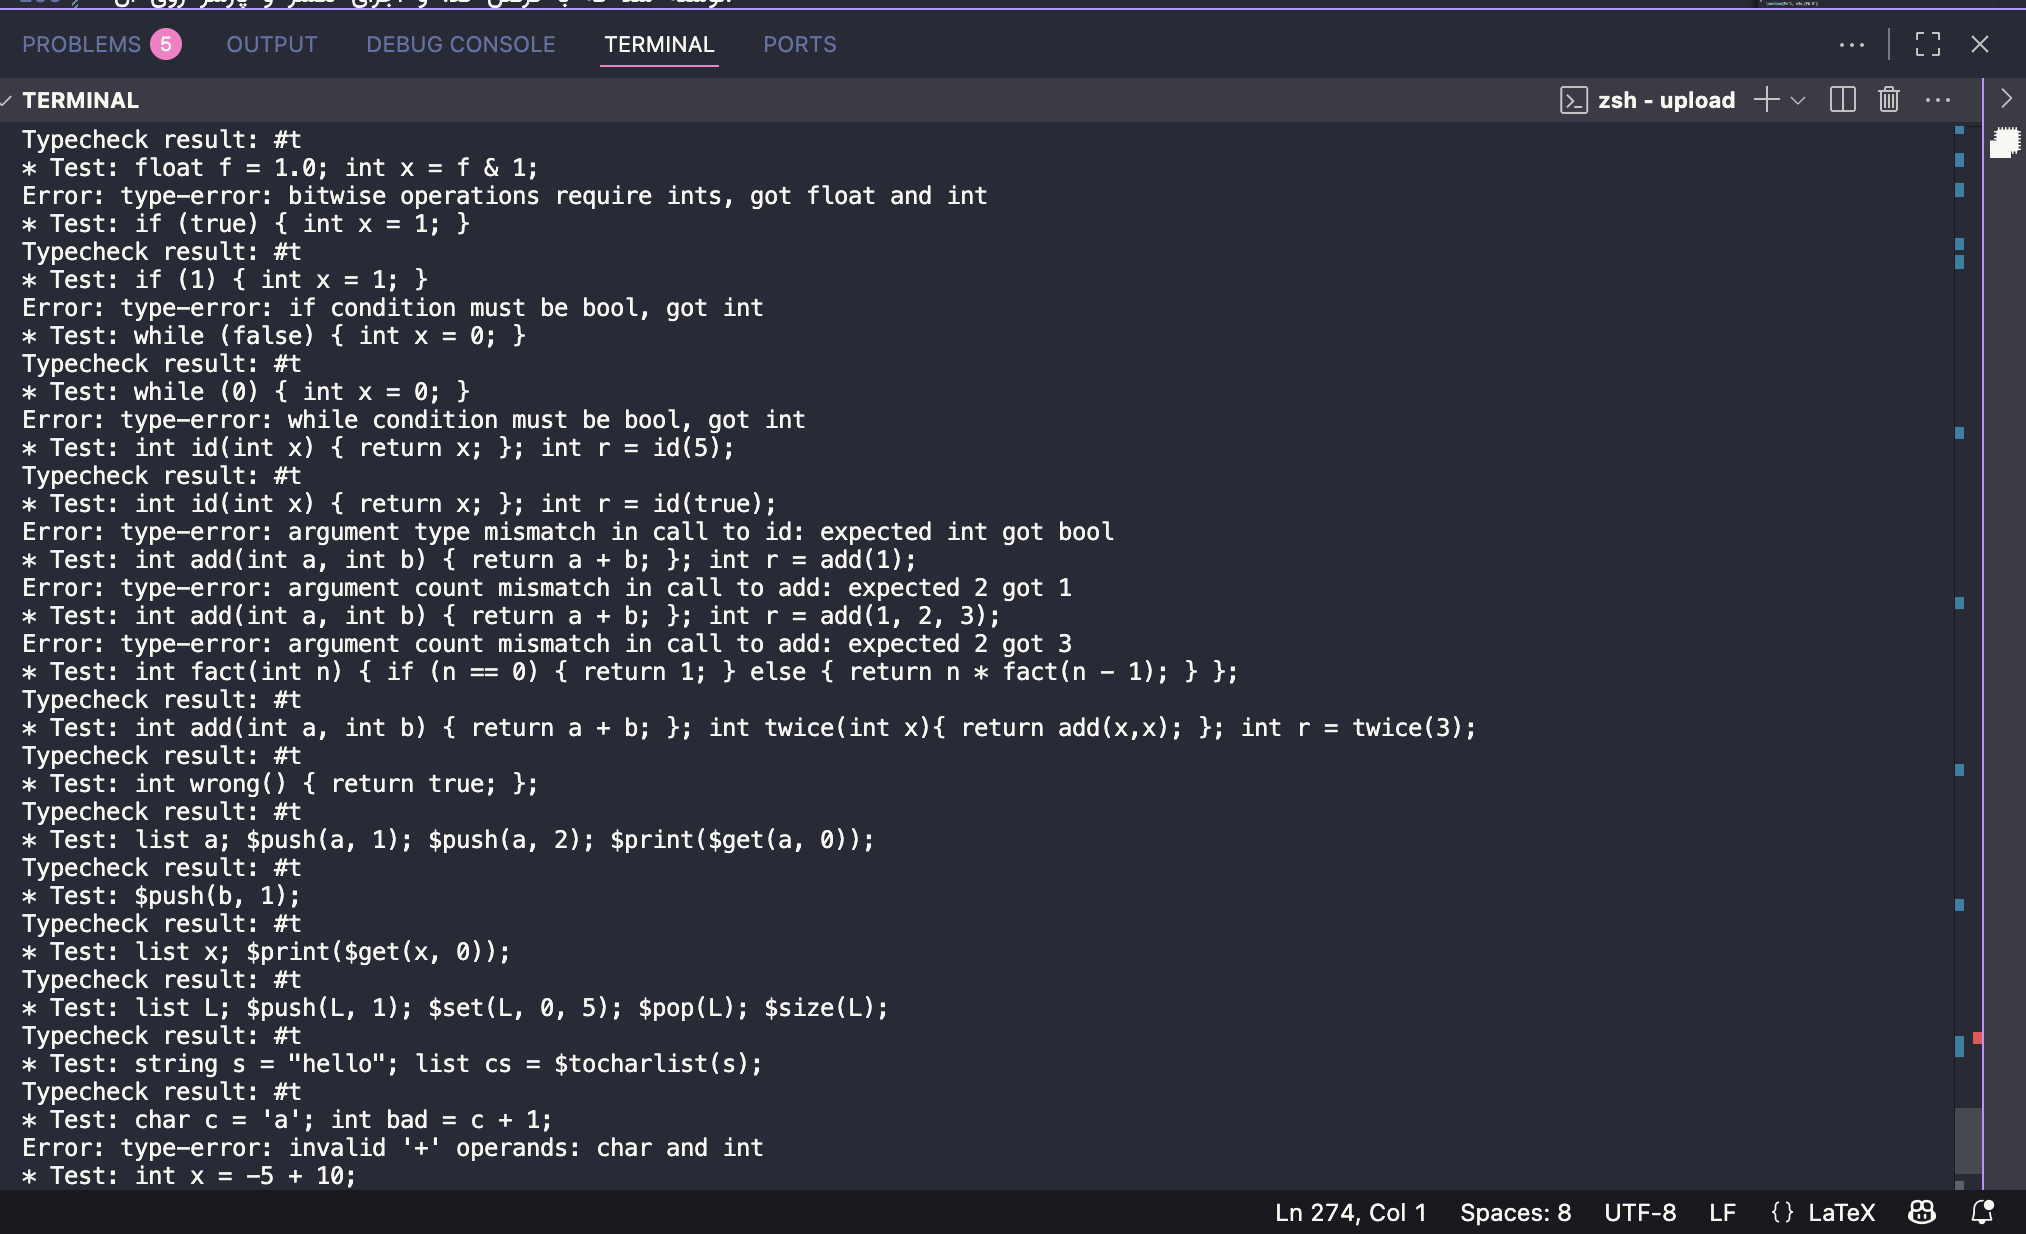
\includegraphics[width=1\linewidth]{pics/tbtc.png}
        \caption{بخشی از خروجی تست‌بنچ تایپ‌چکر}
\end{figure}
\section{نتایج تست‌بنچ ها}
نتایج تست بنچ ها در دایرکتوری 
\texttt{results}
به صورت کامل قابل دسترسیست(همچنین خودتون هم میتونین اجراش کنین طبع :))
\\
عکس از بخش‌هایی از تست‌بنچ‌ها نیز در زیر ضمیمه شده:
\begin{figure}[h]
           \centering
        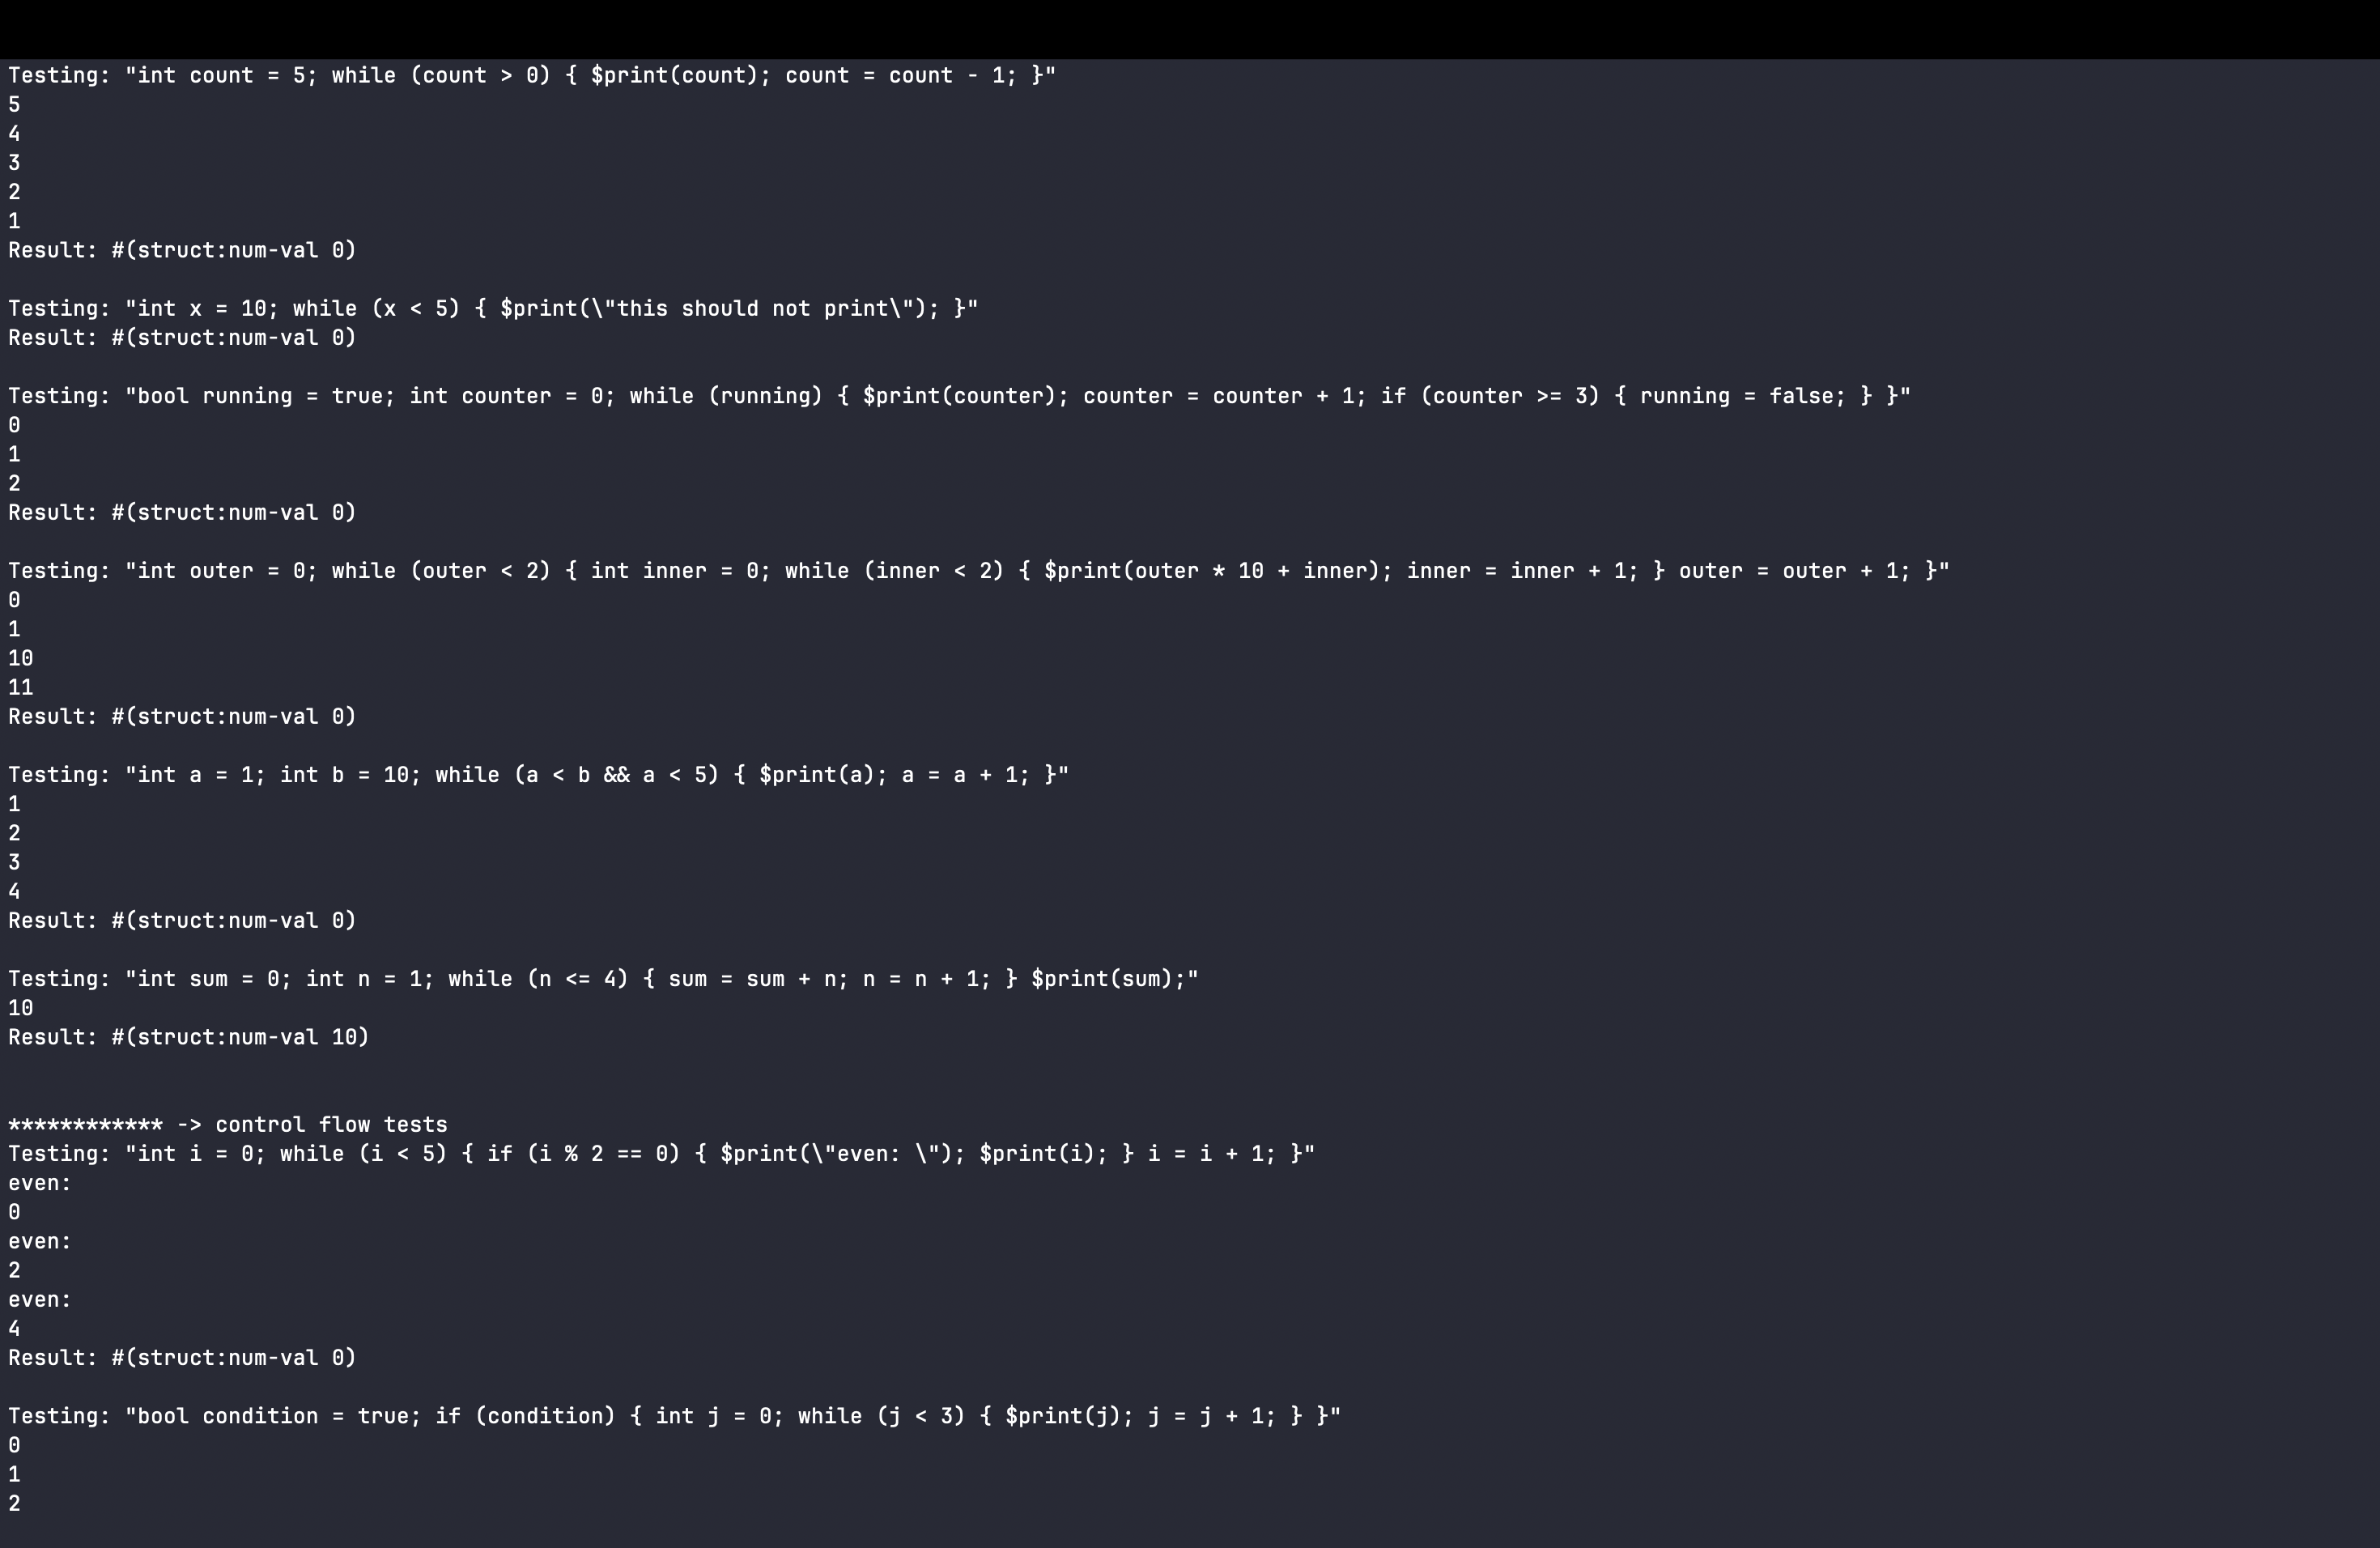
\includegraphics[width=1\linewidth]{pics/basic.png}
        \caption{بخشی از خروجی تست‌بنچ ساده}
\end{figure}
\begin{figure}[h]
           \centering
        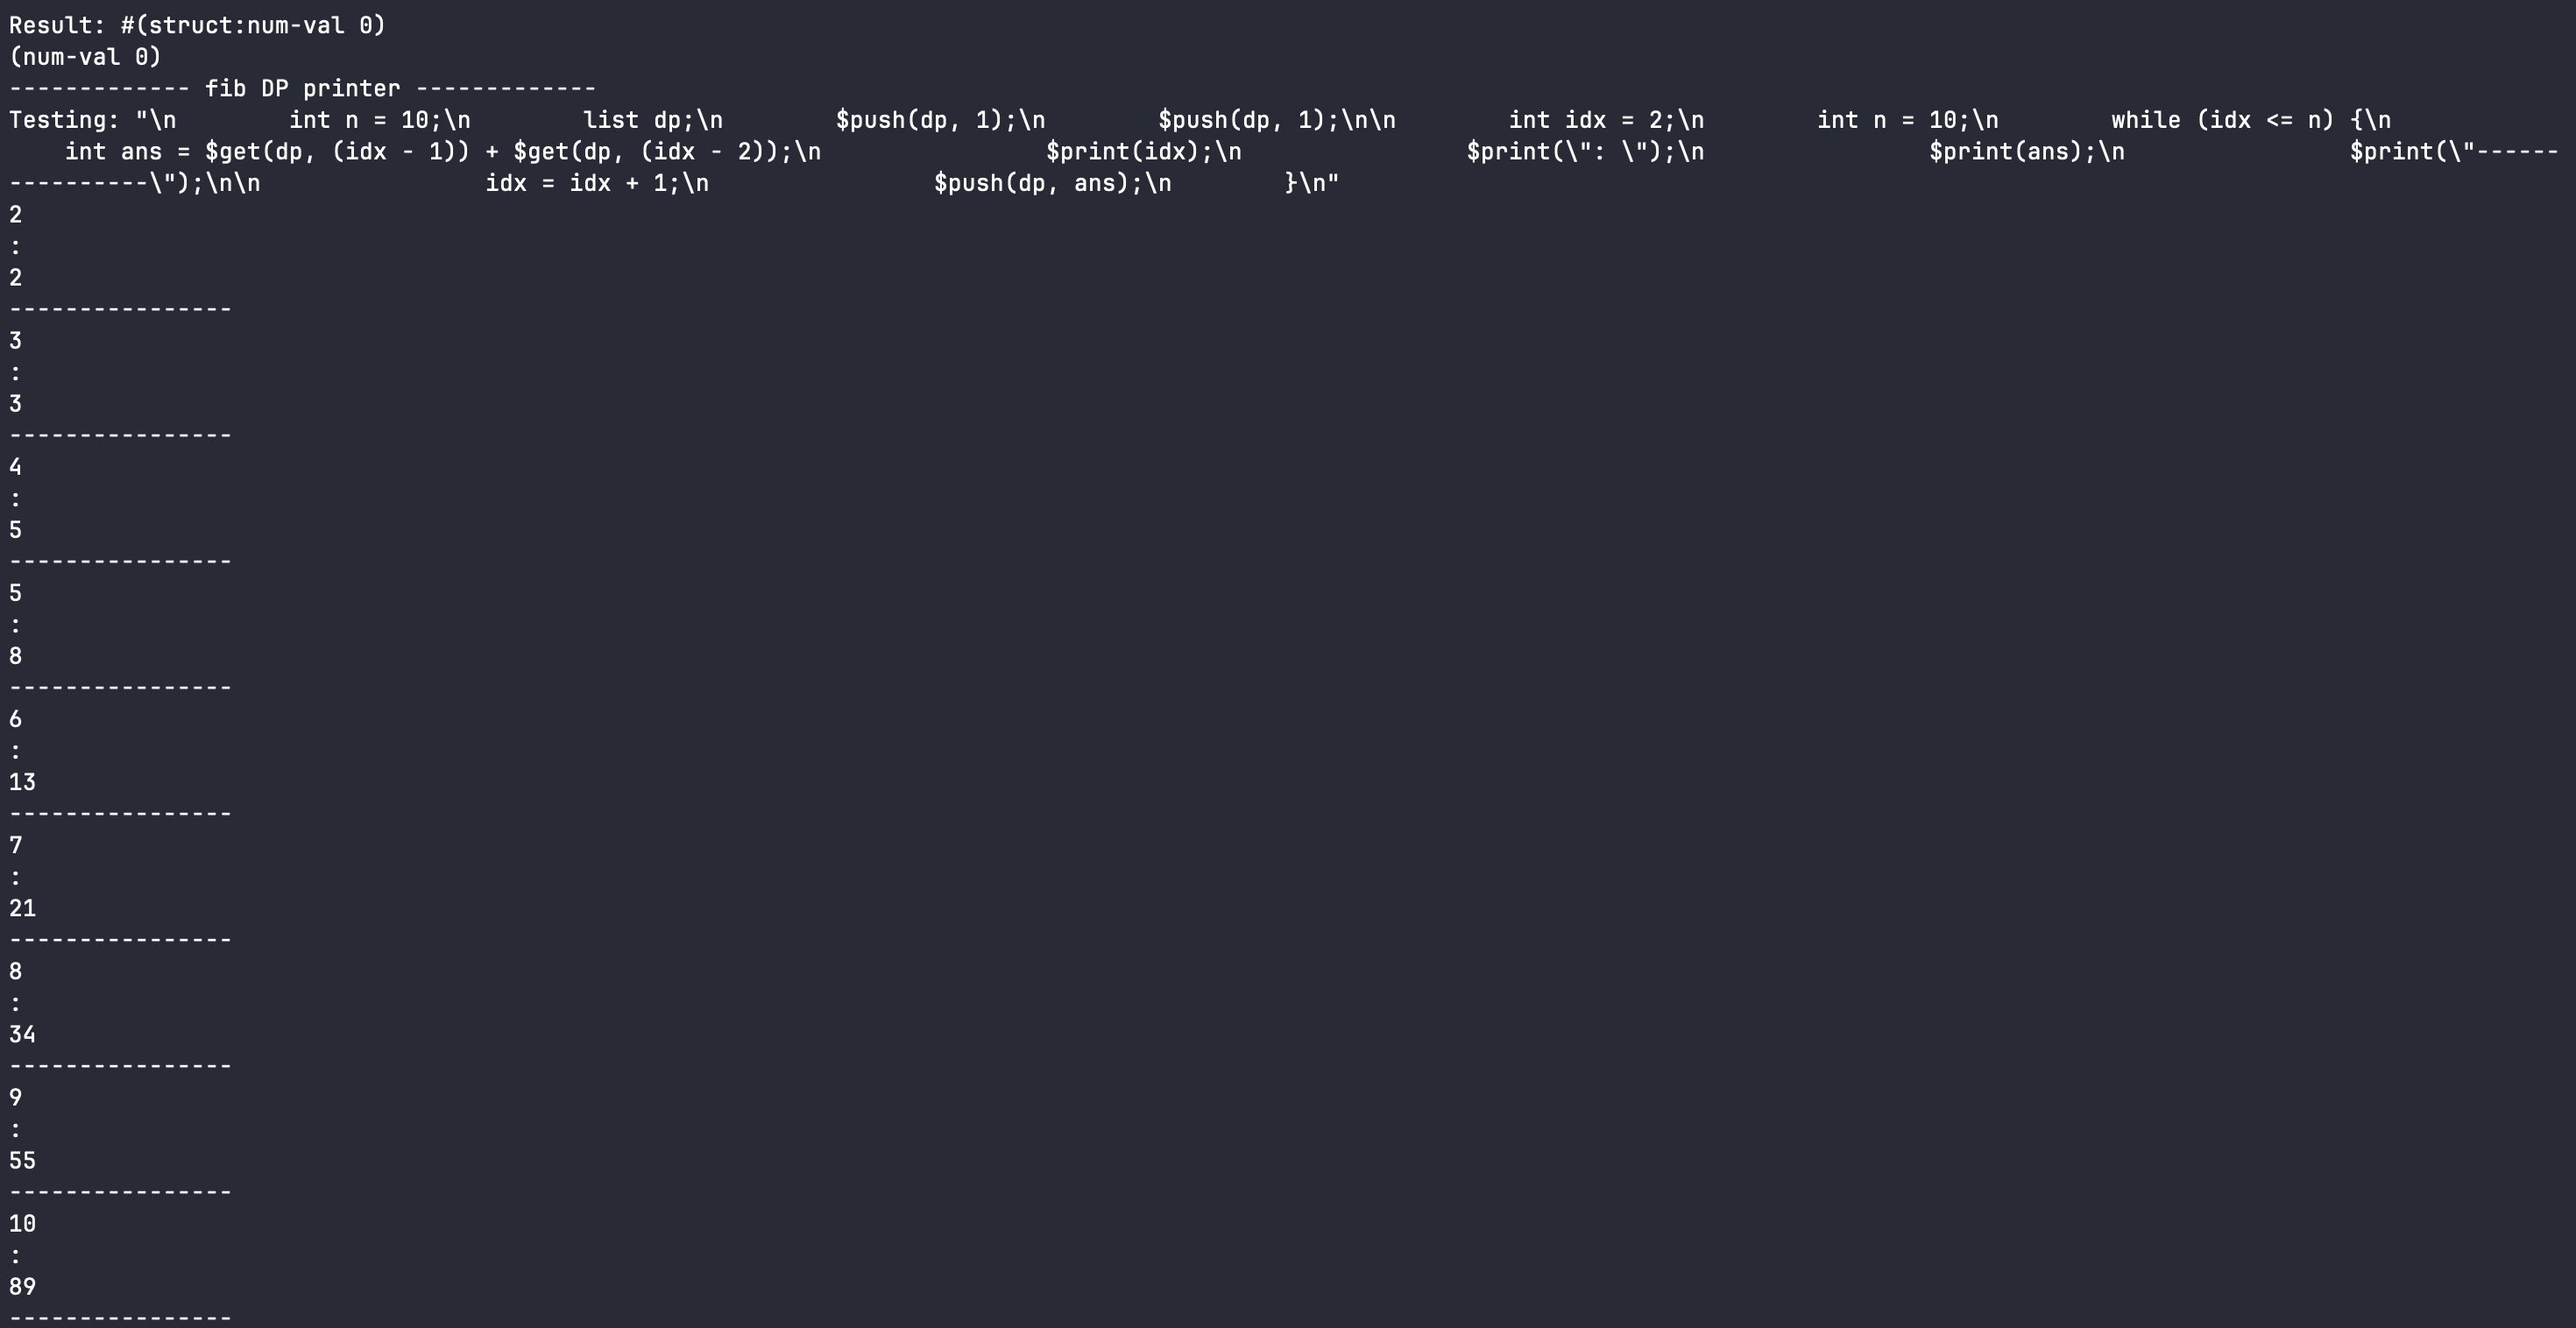
\includegraphics[width=1\linewidth]{pics/fibdp.png}
        \caption{خروجی بخش 10 فیبوناتچی اول به روش بازگشتی تست‌های سخت}
\end{figure}
\begin{figure}[h]
           \centering
        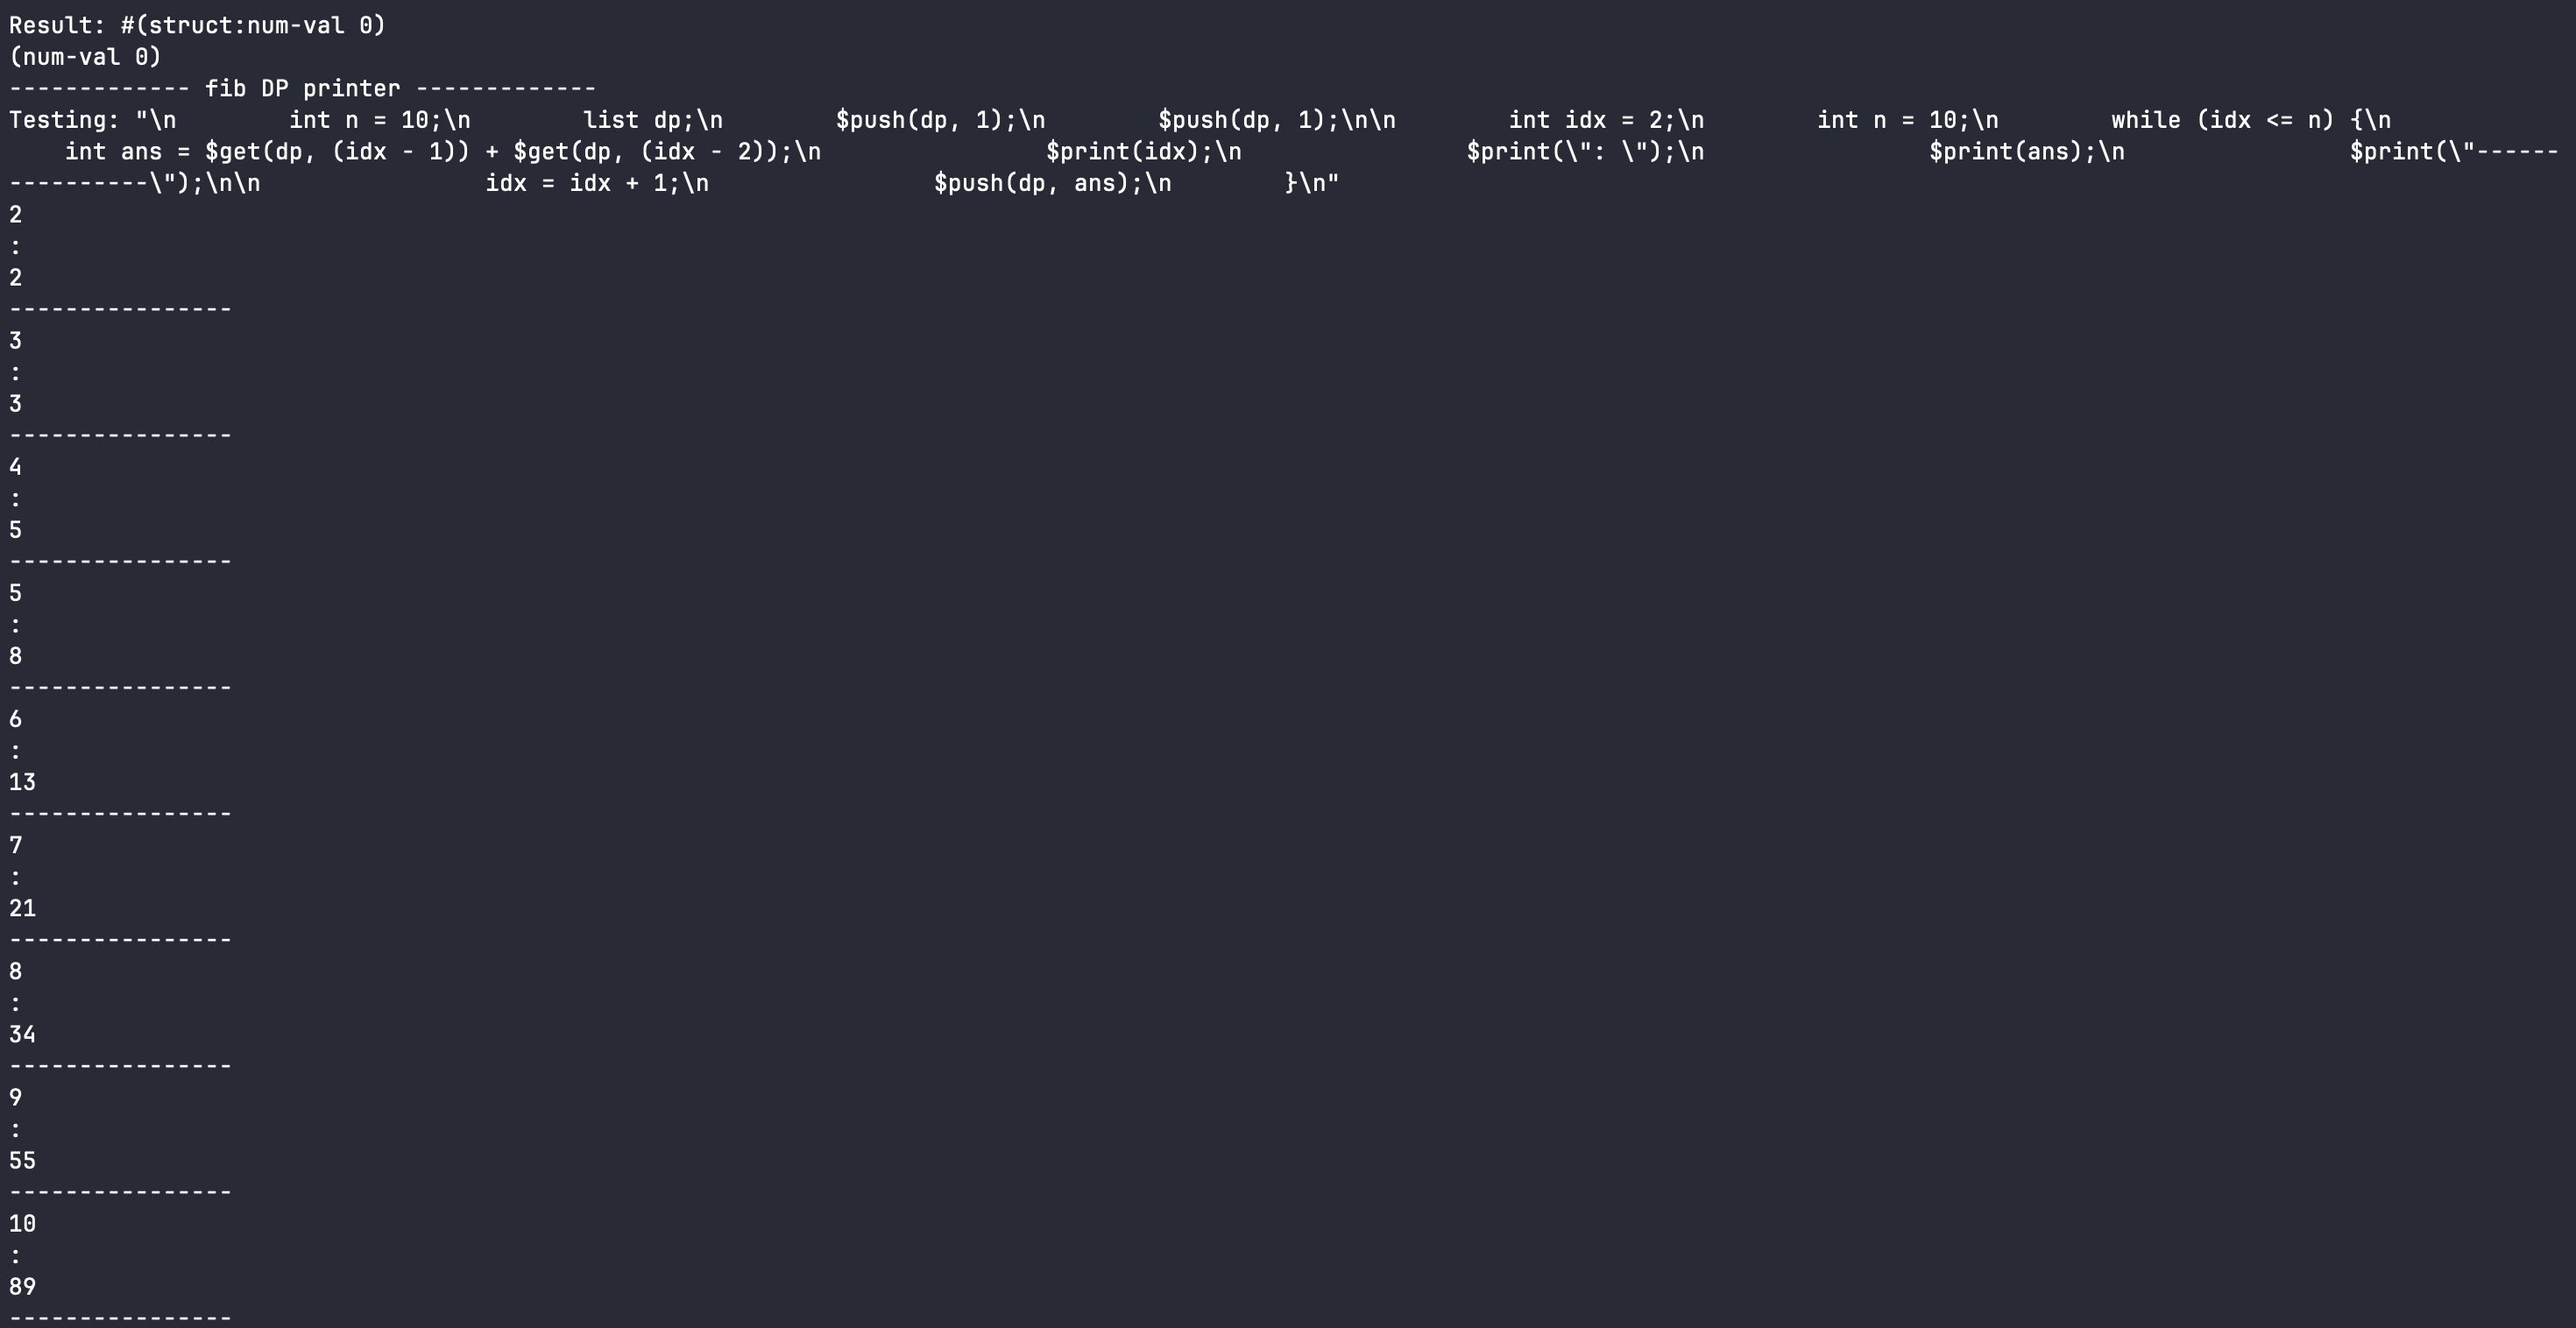
\includegraphics[width=1\linewidth]{pics/fibdp.png}
        \caption{خروجی بخش 10 فیبوناتچی اول به روش دیپی تست‌های سخت}
\end{figure}
\begin{figure}[h]
           \centering
        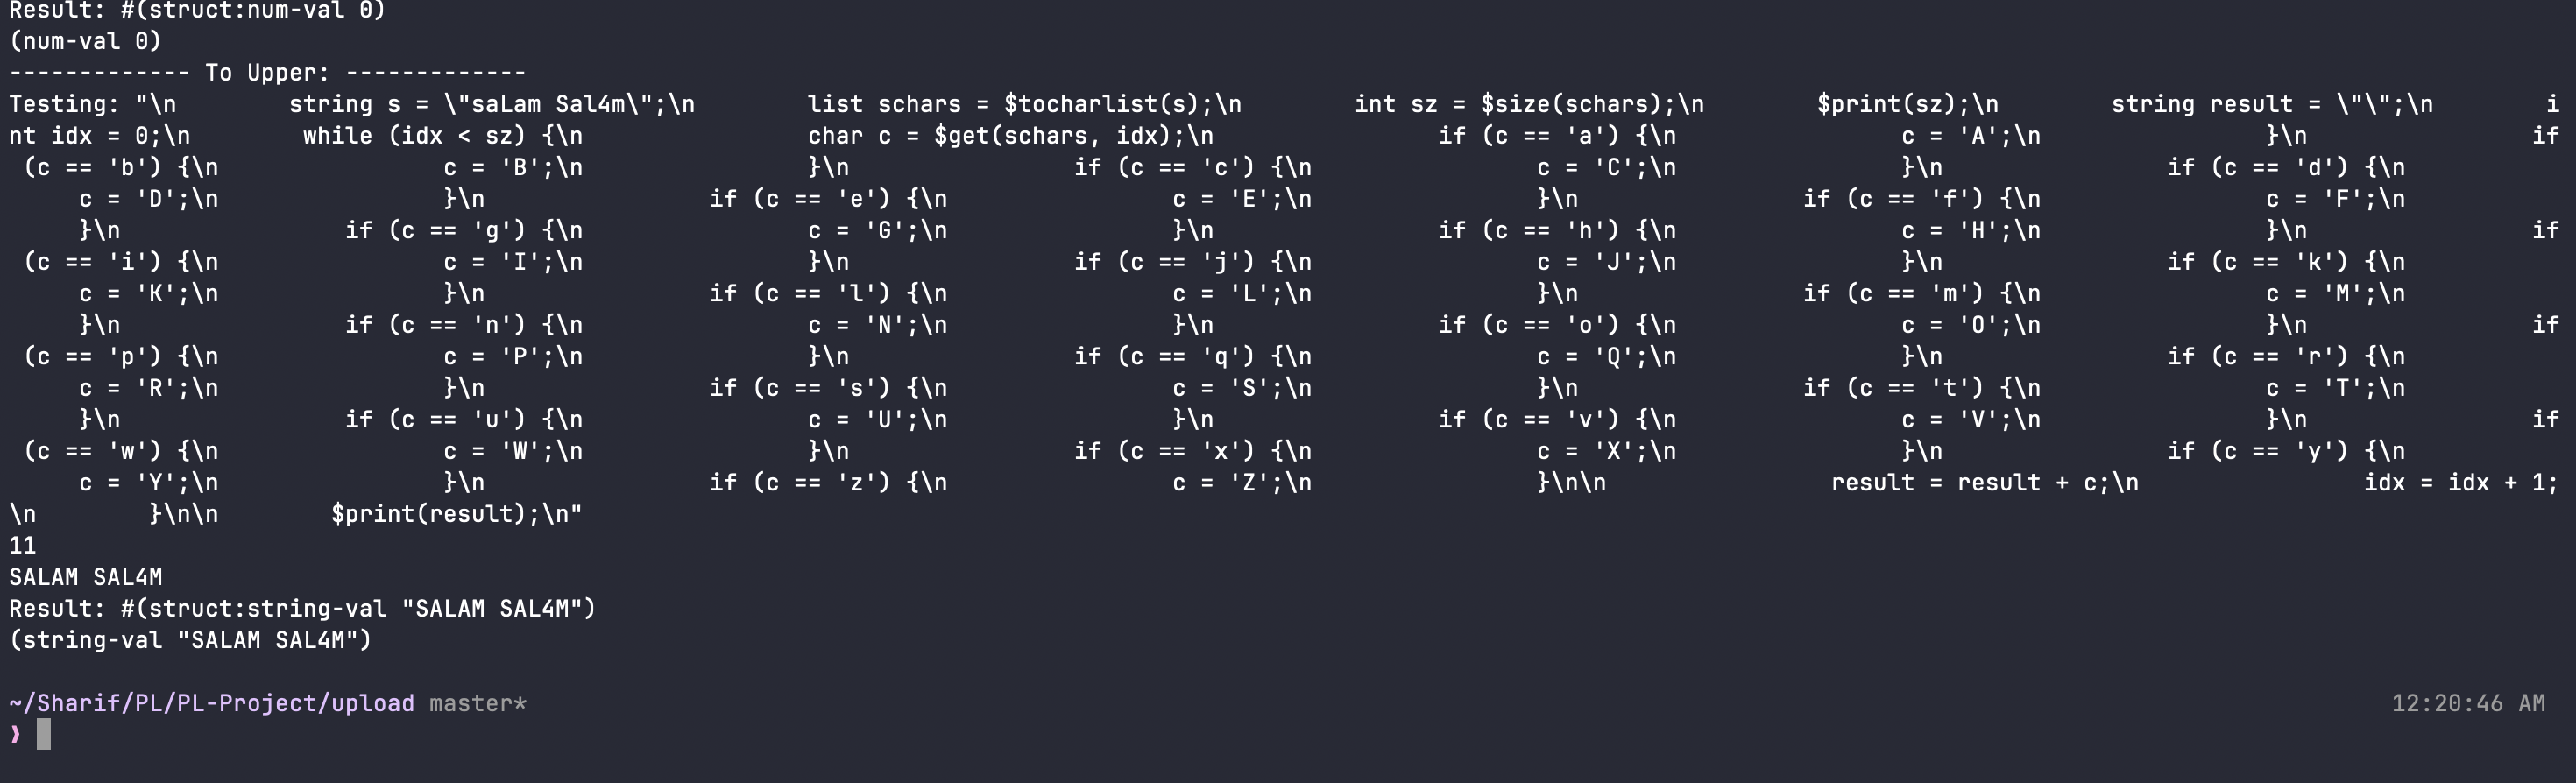
\includegraphics[width=1\linewidth]{pics/toupper.png}
        \caption{خروجی بخش تبدیل به آپرکیس تست‌های سخت}
\end{figure}
\begin{figure}[h]
           \centering
        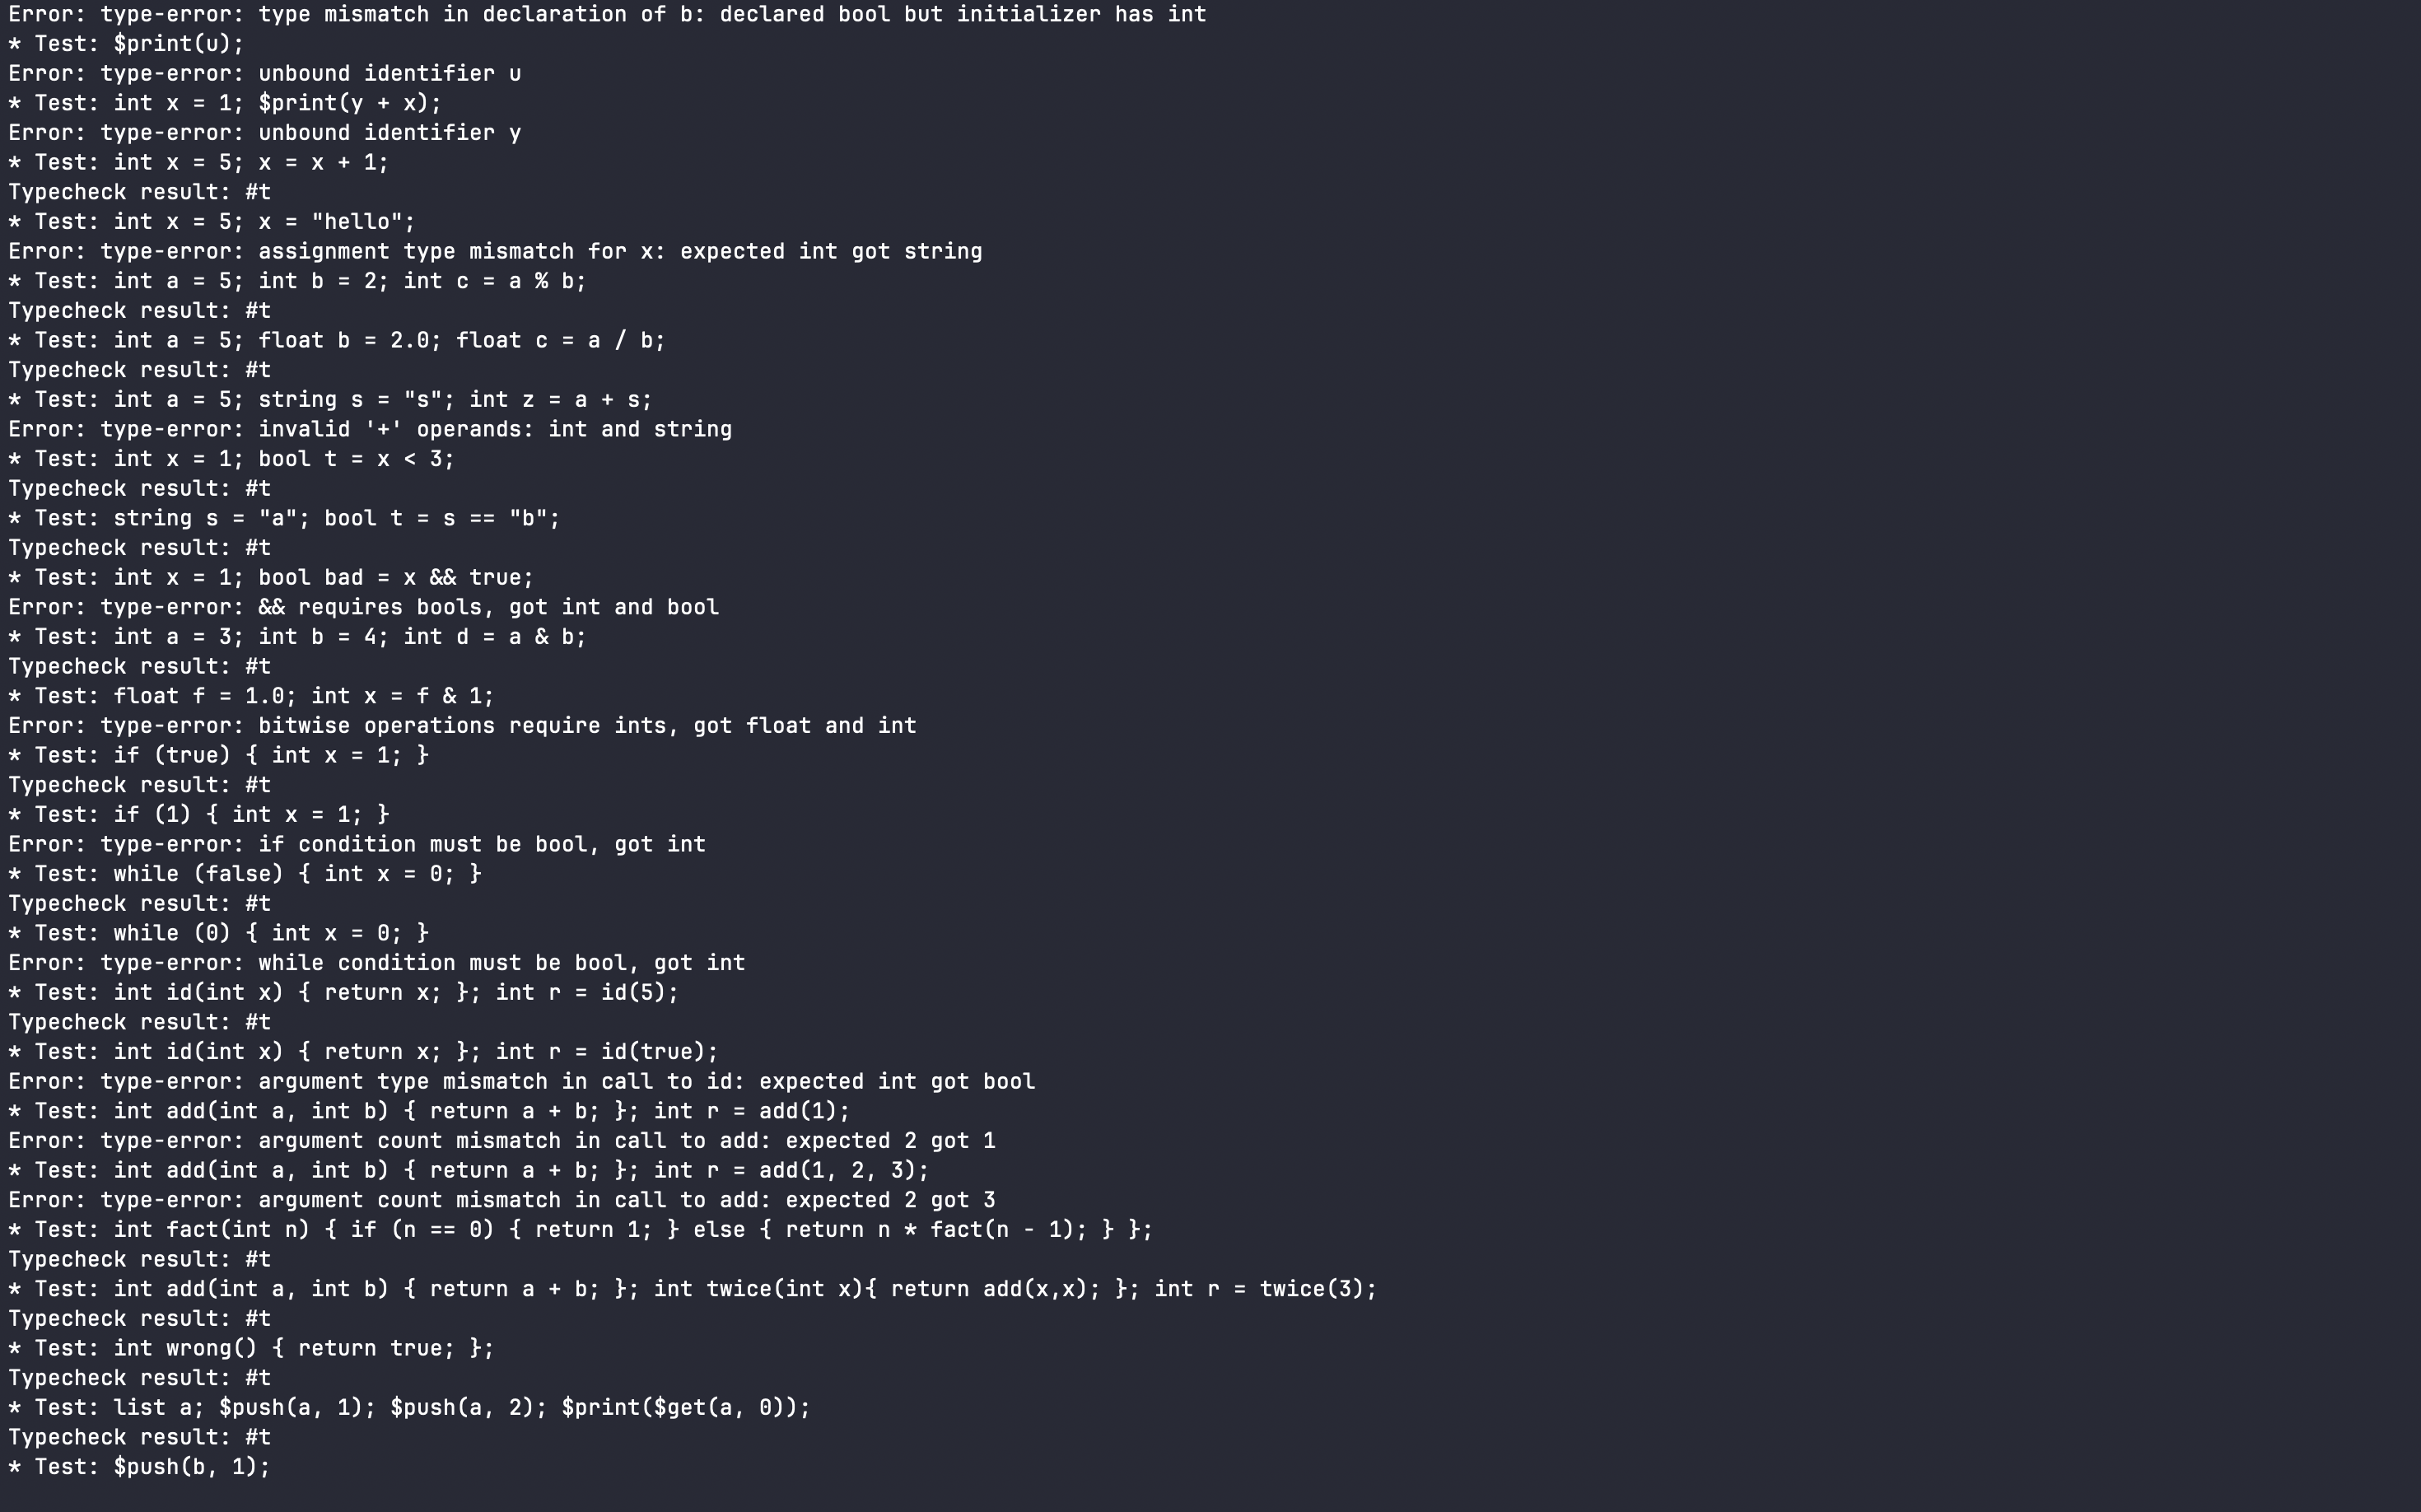
\includegraphics[width=1\linewidth]{pics/test-check.png}
        \caption{بخشی از خروجی تست‌بنچ تایپ‌چکر}
\end{figure}

\FloatBarrier
\end{document}


